% Options for packages loaded elsewhere
\PassOptionsToPackage{unicode}{hyperref}
\PassOptionsToPackage{hyphens}{url}
\PassOptionsToPackage{dvipsnames,svgnames,x11names}{xcolor}
\documentclass[
  10pt,
  a4paper,
]{article}
\usepackage{xcolor}
\usepackage[margin=20mm]{geometry}
\usepackage{amsmath,amssymb}
\usepackage{graphicx}
\graphicspath{{docs/figures/}{figures/}{docs/}{./}}
\setcounter{secnumdepth}{5}
\usepackage{iftex}
\ifPDFTeX
  \usepackage[T1]{fontenc}
  \usepackage[utf8]{inputenc}
  \usepackage{textcomp} % provide euro and other symbols
\else % if luatex or xetex
  \usepackage{unicode-math} % this also loads fontspec
  \defaultfontfeatures{Scale=MatchLowercase}
  \defaultfontfeatures[\rmfamily]{Ligatures=TeX,Scale=1}
\fi
\usepackage{lmodern}
\ifPDFTeX\else
  % xetex/luatex font selection
  \setmainfont[]{Noto Serif}
  \setsansfont[]{Noto Sans}
  \setmonofont[]{DejaVu Sans Mono}
\fi
% Use upquote if available, for straight quotes in verbatim environments
\IfFileExists{upquote.sty}{\usepackage{upquote}}{}
\IfFileExists{microtype.sty}{% use microtype if available
  \usepackage[]{microtype}
  \UseMicrotypeSet[protrusion]{basicmath} % disable protrusion for tt fonts
}{}
\makeatletter
\@ifundefined{KOMAClassName}{% if non-KOMA class
  \IfFileExists{parskip.sty}{%
    \usepackage{parskip}
  }{% else
    \setlength{\parindent}{0pt}
    \setlength{\parskip}{6pt plus 2pt minus 1pt}}
}{% if KOMA class
  \KOMAoptions{parskip=half}}
\makeatother
\usepackage{color}
\usepackage{fancyvrb}
\newcommand{\VerbBar}{|}
\newcommand{\VERB}{\Verb[commandchars=\\\{\}]}
\DefineVerbatimEnvironment{Highlighting}{Verbatim}{commandchars=\\\{\}}
% Add ',fontsize=\small' for more characters per line
\newenvironment{Shaded}{}{}
\newcommand{\AlertTok}[1]{\textcolor[rgb]{1.00,0.00,0.00}{\textbf{#1}}}
\newcommand{\AnnotationTok}[1]{\textcolor[rgb]{0.38,0.63,0.69}{\textbf{\textit{#1}}}}
\newcommand{\AttributeTok}[1]{\textcolor[rgb]{0.49,0.56,0.16}{#1}}
\newcommand{\BaseNTok}[1]{\textcolor[rgb]{0.25,0.63,0.44}{#1}}
\newcommand{\BuiltInTok}[1]{\textcolor[rgb]{0.00,0.50,0.00}{#1}}
\newcommand{\CharTok}[1]{\textcolor[rgb]{0.25,0.44,0.63}{#1}}
\newcommand{\CommentTok}[1]{\textcolor[rgb]{0.38,0.63,0.69}{\textit{#1}}}
\newcommand{\CommentVarTok}[1]{\textcolor[rgb]{0.38,0.63,0.69}{\textbf{\textit{#1}}}}
\newcommand{\ConstantTok}[1]{\textcolor[rgb]{0.53,0.00,0.00}{#1}}
\newcommand{\ControlFlowTok}[1]{\textcolor[rgb]{0.00,0.44,0.13}{\textbf{#1}}}
\newcommand{\DataTypeTok}[1]{\textcolor[rgb]{0.56,0.13,0.00}{#1}}
\newcommand{\DecValTok}[1]{\textcolor[rgb]{0.25,0.63,0.44}{#1}}
\newcommand{\DocumentationTok}[1]{\textcolor[rgb]{0.73,0.13,0.13}{\textit{#1}}}
\newcommand{\ErrorTok}[1]{\textcolor[rgb]{1.00,0.00,0.00}{\textbf{#1}}}
\newcommand{\ExtensionTok}[1]{#1}
\newcommand{\FloatTok}[1]{\textcolor[rgb]{0.25,0.63,0.44}{#1}}
\newcommand{\FunctionTok}[1]{\textcolor[rgb]{0.02,0.16,0.49}{#1}}
\newcommand{\ImportTok}[1]{\textcolor[rgb]{0.00,0.50,0.00}{\textbf{#1}}}
\newcommand{\InformationTok}[1]{\textcolor[rgb]{0.38,0.63,0.69}{\textbf{\textit{#1}}}}
\newcommand{\KeywordTok}[1]{\textcolor[rgb]{0.00,0.44,0.13}{\textbf{#1}}}
\newcommand{\NormalTok}[1]{#1}
\newcommand{\OperatorTok}[1]{\textcolor[rgb]{0.40,0.40,0.40}{#1}}
\newcommand{\OtherTok}[1]{\textcolor[rgb]{0.00,0.44,0.13}{#1}}
\newcommand{\PreprocessorTok}[1]{\textcolor[rgb]{0.74,0.48,0.00}{#1}}
\newcommand{\RegionMarkerTok}[1]{#1}
\newcommand{\SpecialCharTok}[1]{\textcolor[rgb]{0.25,0.44,0.63}{#1}}
\newcommand{\SpecialStringTok}[1]{\textcolor[rgb]{0.73,0.40,0.53}{#1}}
\newcommand{\StringTok}[1]{\textcolor[rgb]{0.25,0.44,0.63}{#1}}
\newcommand{\VariableTok}[1]{\textcolor[rgb]{0.10,0.09,0.49}{#1}}
\newcommand{\VerbatimStringTok}[1]{\textcolor[rgb]{0.25,0.44,0.63}{#1}}
\newcommand{\WarningTok}[1]{\textcolor[rgb]{0.38,0.63,0.69}{\textbf{\textit{#1}}}}
\usepackage{longtable,booktabs,array}
\usepackage{calc} % for calculating minipage widths
\newcolumntype{L}[1]{>{\raggedright\arraybackslash\sloppy}p{#1}}
% Correct order of tables after \paragraph or \subparagraph
\usepackage{etoolbox}
\makeatletter
\patchcmd\longtable{\par}{\if@noskipsec\mbox{}\fi\par}{}{}
\makeatother
\AtBeginEnvironment{longtable}{\small}
\setlength\LTleft{0pt}
\setlength\LTright{0pt}
% Allow footnotes in longtable head/foot
\IfFileExists{footnotehyper.sty}{\usepackage{footnotehyper}}{\usepackage{footnote}}
\makesavenoteenv{longtable}
\setlength{\emergencystretch}{3em} % prevent overfull lines
\providecommand{\tightlist}{%
  \setlength{\itemsep}{0pt}\setlength{\parskip}{0pt}}
\usepackage{bookmark}
\IfFileExists{xurl.sty}{\usepackage{xurl}}{} % add URL line breaks if available
\urlstyle{same}
\hypersetup{
  pdftitle={MBS-fast Manual},
  colorlinks=true,
  linkcolor={blue},
  filecolor={Maroon},
  citecolor={Blue},
  urlcolor={blue},
  pdfcreator={LaTeX via pandoc}}

\title{MBS-fast Manual}
\author{}
\date{August 12, 2026}

\begin{document}
\maketitle

\renewcommand*\contentsname{Contents}
{
\setcounter{tocdepth}{3}
\tableofcontents
}
MBS-fast computes light scattering by non-spherical particles with
geometrical ray tracing plus Physical Optics (PO) diffraction. The code
is optimized for CPU OpenMP/MPI runs and CUDA GPU diffraction runs. This
manual describes the current command line interface, build targets,
grids, multi-GPU scans, and the main diffraction/Jones/Mueller formulas
used by the implementation.

\section{Build}\label{build}

\subsection{Requirements}\label{requirements}

\begin{longtable}[]{@{}L{0.24\linewidth}L{0.28\linewidth}L{0.40\linewidth}@{}}
\toprule\noalign{}
Component & Required for & Notes \\
\midrule\noalign{}
\endhead
\bottomrule\noalign{}
\endlastfoot
GCC \textgreater= 9 or Clang \textgreater= 14 & CPU and host CUDA code &
GCC is the normal path on EPYC \\
OpenMP & CPU parallelism & GCC links with \texttt{libgomp} \\
MPI & \texttt{cpu/} split build & \texttt{mpicxx} is used when
available \\
CUDA toolkit & \texttt{gpu/} split build & \texttt{nvcc},
\texttt{libcudart}, \texttt{libcufft} \\
NVIDIA driver & GPU runs & Must support the requested \texttt{sm\_XX}
binary \\
\end{longtable}

The split build is the recommended build path. CPU objects are kept
under \texttt{cpu/build/}; CUDA objects are kept under
\texttt{gpu/build/}. The shared physics code remains in \texttt{src/}.

\subsection{CPU build}\label{cpu-build}

\begin{Shaded}
\begin{Highlighting}[]
\CommentTok{\# MPI + OpenMP CPU binary}
\FunctionTok{make} \AttributeTok{{-}C}\NormalTok{ cpu }\AttributeTok{{-}j}

\CommentTok{\# Run one MPI rank with 64 OpenMP threads}
\VariableTok{OMP\_NUM\_THREADS}\OperatorTok{=}\NormalTok{64 }\ExtensionTok{cpu/bin/mbs\_po\_mpi} \AttributeTok{{-}{-}po} \AttributeTok{{-}p}\NormalTok{ 1 125.9 78.09 }\DataTypeTok{\textbackslash{}}
    \AttributeTok{{-}{-}ri}\NormalTok{ 1.3116 0 }\AttributeTok{{-}w}\NormalTok{ 0.532 }\AttributeTok{{-}n}\NormalTok{ 12 }\AttributeTok{{-}{-}oldauto}\NormalTok{ 2 }\DataTypeTok{\textbackslash{}}
    \AttributeTok{{-}{-}grid}\NormalTok{ 0 180 600 180 }\AttributeTok{{-}{-}threads}\NormalTok{ 64 }\AttributeTok{{-}{-}close} \AttributeTok{{-}o}\NormalTok{ out\_cpu}

\CommentTok{\# Run four MPI ranks, each with 16 OpenMP threads}
\ExtensionTok{mpirun} \AttributeTok{{-}np}\NormalTok{ 4 cpu/bin/mbs\_po\_mpi }\AttributeTok{{-}{-}po} \AttributeTok{{-}p}\NormalTok{ 1 125.9 78.09 }\DataTypeTok{\textbackslash{}}
    \AttributeTok{{-}{-}ri}\NormalTok{ 1.3116 0 }\AttributeTok{{-}w}\NormalTok{ 0.532 }\AttributeTok{{-}n}\NormalTok{ 12 }\AttributeTok{{-}{-}oldauto}\NormalTok{ 2 }\DataTypeTok{\textbackslash{}}
    \AttributeTok{{-}{-}grid}\NormalTok{ 0 180 600 180 }\AttributeTok{{-}{-}threads}\NormalTok{ 16 }\AttributeTok{{-}{-}close} \AttributeTok{{-}o}\NormalTok{ out\_cpu\_mpi}
\end{Highlighting}
\end{Shaded}

Debug help build:

\begin{Shaded}
\begin{Highlighting}[]
\FunctionTok{make} \AttributeTok{{-}C}\NormalTok{ cpu debug}
\ExtensionTok{cpu/bin/mbs\_po\_mpi\_debug} \AttributeTok{{-}{-}help{-}debug}
\end{Highlighting}
\end{Shaded}

\subsection{GPU build}\label{gpu-build}

\begin{Shaded}
\begin{Highlighting}[]
\CommentTok{\# Default/reference GPU binary: FP64 with precise math}
\VariableTok{PATH}\OperatorTok{=}\NormalTok{/usr/local/cuda/bin:}\VariableTok{$PATH} \FunctionTok{make} \AttributeTok{{-}C}\NormalTok{ gpu }\AttributeTok{{-}j}

\CommentTok{\# Explicit variants}
\FunctionTok{make} \AttributeTok{{-}C}\NormalTok{ gpu fp32      }\AttributeTok{{-}j}   \CommentTok{\# gpu/bin/mbs\_po\_gpu\_float}
\FunctionTok{make} \AttributeTok{{-}C}\NormalTok{ gpu fp32\_consumer }\AttributeTok{{-}j} \CommentTok{\# gpu/bin/mbs\_po\_gpu\_float\_consumer}
\FunctionTok{make} \AttributeTok{{-}C}\NormalTok{ gpu fp64      }\AttributeTok{{-}j}   \CommentTok{\# gpu/bin/mbs\_po\_gpu\_double}
\FunctionTok{make} \AttributeTok{{-}C}\NormalTok{ gpu fp32\_fast }\AttributeTok{{-}j}   \CommentTok{\# gpu/bin/mbs\_po\_gpu\_float\_fast}
\FunctionTok{make} \AttributeTok{{-}C}\NormalTok{ gpu fp64\_fast }\AttributeTok{{-}j}   \CommentTok{\# gpu/bin/mbs\_po\_gpu\_double\_fast}
\end{Highlighting}
\end{Shaded}

\begin{longtable}[]{@{}L{0.20\linewidth}L{0.32\linewidth}L{0.10\linewidth}L{0.10\linewidth}L{0.18\linewidth}@{}}
\toprule\noalign{}
Target & Binary & CUDA precision & Fast math & Typical use \\
\midrule\noalign{}
\endhead
\bottomrule\noalign{}
\endlastfoot
\texttt{make\ -C\ gpu} or \texttt{make\ -C\ gpu\ fp64} &
\nolinkurl{gpu/bin/mbs_po_gpu_double} & FP64 & no & Numerical reference and production default \\
\texttt{make\ -C\ gpu\ fp32} & \nolinkurl{gpu/bin/mbs_po_gpu_float} &
FP32 & no & Calibrated FP32 throughput \\
\texttt{make\ -C\ gpu\ fp32\_consumer} &
\nolinkurl{gpu/bin/mbs_po_gpu_float_consumer} & FP32 & no & Consumer GPU throughput with FP32 phase trigonometry \\
\texttt{make\ -C\ gpu\ fp32\_fast} &
\nolinkurl{gpu/bin/mbs_po_gpu_float_fast} & FP32 & yes & Experimental profile; benchmark after validation \\
\texttt{make\ -C\ gpu\ fp64\_fast} &
\nolinkurl{gpu/bin/mbs_po_gpu_double_fast} & FP64 & yes & FP64 throughput after validation \\
\texttt{make\ -C\ gpu\ double\_debug} &
\nolinkurl{gpu/bin/mbs_po_gpu_double_debug} & FP64 & yes & Debug help
and diagnostics \\
\end{longtable}

The low-level build variable is
\texttt{GPU\_PHASE\_TRIG=precise|consumer}. The consumer value is valid only
with FP32 storage, has a separate object directory, and does not enable
\texttt{-{}-use\_fast\_math}. The supported shortcut is
\texttt{make -C gpu fp32\_consumer -j}. Run
\texttt{make test\_cuda\_consumer} on the target GPU after building.

FP32 applies to diffraction-beam storage, Jones sums, and Mueller output.
Visibility/topology tracing, optical paths, absorption, cancellation-prone
polygon moments, and phase construction remain FP64. The precise FP32 binary
also evaluates phase trigonometry in FP64. The consumer binary casts only the
completed phase to FP32 for \texttt{sincosf}. \texttt{-{}-version} reports
both phase precisions, the math profile, and target architecture.

Verify every rebuilt binary before starting a queue:

\begin{verbatim}
gpu/bin/mbs_po_gpu_double --version  # fp64-diffraction-storage ... precise-math
gpu/bin/mbs_po_gpu_float --version   # fp32-diffraction-storage ... precise-math
gpu/bin/mbs_po_gpu_float_consumer --version  # phase-build-fp64 phase-trig-fp32
\end{verbatim}

CUDA host compilation requires exactly one FP32/FP64 profile. A binary that
reports \texttt{unknown-precision} is stale or was built outside the supported
profiles and must not be used for production calculations.

On an RTX 3080 Ti, a representative absorbing nonconvex test
($L=20\ \mu\mathrm{m}$, 192 SO(3) orientations,
$N_\phi=288$, $N_\theta=144$) gave the following medians:

\begin{longtable}[]{@{}L{0.28\linewidth}L{0.18\linewidth}L{0.18\linewidth}L{0.24\linewidth}@{}}
\toprule\noalign{}
Profile & Time & Speedup over FP64 & Mueller error against FP64 \\
\midrule\noalign{}
\endhead
\bottomrule\noalign{}
\endlastfoot
Precise FP64 & 8.56 s & 1.00 & reference \\
Precise mixed FP32 & 5.76 s & 1.49 & global $L_2=5.68\times10^{-8}$ \\
Consumer FP32 & 3.25 s & 2.63 & global $L_2=2.82\times10^{-7}$ \\
\end{longtable}

After calibration, the consumer FP32 binary is the recommended throughput
profile. It was 1.77 times faster than precise mixed FP32. Across convex,
concave, absorbing, nonabsorbing, $L=5\ldots500\ \mu\mathrm{m}$, and 8--20
reflection probes, the largest side/back M11 L2 error was $8.4\times10^{-5}$;
one weak off-diagonal element reached $5.3\times10^{-3}$. Whole-kernel fast
math was about 9\% slower than the consumer profile. Final reference points
and numerically sensitive cases should still be checked in FP64.

The GPU split build enables CUDA diffraction by default.
\texttt{-\/-gpu} is accepted but optional. Use \texttt{-\/-cpu} only
when you deliberately want the CPU diffraction backend from a
GPU-capable binary.

The Makefile detects the GPU compute capability with
\texttt{nvidia-smi}. Override when needed:

\begin{Shaded}
\begin{Highlighting}[]
\CommentTok{\# Ampere, e.g. RTX 3080 Ti}
\FunctionTok{make} \AttributeTok{{-}C}\NormalTok{ gpu fp32\_consumer }\AttributeTok{{-}j}\NormalTok{ GPU\_ARCH=86}

\CommentTok{\# Ada, e.g. RTX 4070}
\FunctionTok{make} \AttributeTok{{-}C}\NormalTok{ gpu fp32 }\AttributeTok{{-}j}\NormalTok{ GPU\_ARCH=89}
\end{Highlighting}
\end{Shaded}

\subsection{EPYC Zen5, AVX-512, and
AVX2}\label{epyc-zen5-avx-512-and-avx2}

\texttt{scripts/detect\_arch\_flags.sh} is used by the Makefiles through
\texttt{ARCH\_FLAGS}. On a native machine, the safest high-performance
option is usually:

\begin{Shaded}
\begin{Highlighting}[]
\FunctionTok{make} \AttributeTok{{-}C}\NormalTok{ cpu clean}
\FunctionTok{make} \AttributeTok{{-}C}\NormalTok{ cpu }\AttributeTok{{-}j}\NormalTok{ ARCH\_FLAGS=}\StringTok{"{-}march=native {-}mtune=native"}

\FunctionTok{make} \AttributeTok{{-}C}\NormalTok{ gpu clean}
\FunctionTok{make} \AttributeTok{{-}C}\NormalTok{ gpu double\_fast }\AttributeTok{{-}j}\NormalTok{ ARCH\_FLAGS=}\StringTok{"{-}march=native {-}mtune=native"}
\end{Highlighting}
\end{Shaded}

For named AMD targets:

\begin{longtable}[]{@{}L{0.24\linewidth}L{0.28\linewidth}L{0.40\linewidth}@{}}
\toprule\noalign{}
CPU target & GCC/Clang flags & Notes \\
\midrule\noalign{}
\endhead
\bottomrule\noalign{}
\endlastfoot
EPYC Zen2 & \texttt{ARCH\_FLAGS="-march=znver2\ -mtune=znver2"} &
AVX2/FMA path \\
EPYC Zen3 & \texttt{ARCH\_FLAGS="-march=znver3\ -mtune=znver3"} &
AVX2/FMA path \\
EPYC Zen4 & \texttt{ARCH\_FLAGS="-march=znver4\ -mtune=znver4"} &
AVX-512 capable on GCC versions that support it \\
EPYC Zen5 & \texttt{ARCH\_FLAGS="-march=znver5\ -mtune=znver5"} & Use
with a compiler that knows \texttt{znver5} \\
Portable AVX2 & \texttt{ARCH\_FLAGS="-O3\ -mavx2\ -mfma"} & Runs on AVX2
machines \\
Explicit AVX-512 &
\texttt{ARCH\_FLAGS="-O3\ -mavx512f\ -mavx512dq\ -mavx512cd\ -mavx512bw\ -mavx512vl"}
& Use only on machines that support these flags \\
\end{longtable}

There is no GCC/Clang option named \texttt{AVX12}. If the intended
target is Zen5 with AVX-512, use \texttt{-march=znver5} when the
compiler supports it. If the compiler is older, either upgrade GCC/Clang
or use the explicit AVX-512 flags above after checking
\texttt{lscpu\ \textbar{}\ grep\ avx512}.

\subsection{Legacy root Makefile}\label{legacy-root-makefile}

The root \texttt{Makefile} still exists for compatibility:

\begin{Shaded}
\begin{Highlighting}[]
\FunctionTok{make}                         \CommentTok{\# bin/mbs\_po, CPU}
\FunctionTok{make}\NormalTok{ gpu\_double\_fast         }\CommentTok{\# delegates to gpu/double\_fast}
\FunctionTok{make}\NormalTok{ gpu\_float\_fast          }\CommentTok{\# delegates to gpu/float\_fast}
\FunctionTok{make}\NormalTok{ USE\_CUDA=1              }\CommentTok{\# legacy single{-}tree CUDA build}
\end{Highlighting}
\end{Shaded}

Prefer the split \texttt{cpu/} and \texttt{gpu/} builds for normal work.

\section{Quick runs}\label{quick-runs}

\begin{Shaded}
\begin{Highlighting}[]
\CommentTok{\# GPU double, oldauto orientation grid, full 0..180 degree output}
\ExtensionTok{gpu/bin/mbs\_po\_gpu\_double\_fast} \AttributeTok{{-}{-}po} \AttributeTok{{-}p}\NormalTok{ 1 125.9 78.09 }\DataTypeTok{\textbackslash{}}
    \AttributeTok{{-}{-}ri}\NormalTok{ 1.3116 0 }\AttributeTok{{-}w}\NormalTok{ 0.532 }\AttributeTok{{-}n}\NormalTok{ 12 }\AttributeTok{{-}{-}oldauto}\NormalTok{ 2 }\DataTypeTok{\textbackslash{}}
    \AttributeTok{{-}{-}grid}\NormalTok{ 0 180 600 180 }\AttributeTok{{-}{-}threads}\NormalTok{ 64 }\AttributeTok{{-}{-}close} \AttributeTok{{-}o}\NormalTok{ hex\_gpu\_double}

\CommentTok{\# Same run, force CPU backend from the GPU binary}
\ExtensionTok{gpu/bin/mbs\_po\_gpu\_double\_fast} \AttributeTok{{-}{-}po} \AttributeTok{{-}{-}cpu} \AttributeTok{{-}p}\NormalTok{ 1 125.9 78.09 }\DataTypeTok{\textbackslash{}}
    \AttributeTok{{-}{-}ri}\NormalTok{ 1.3116 0 }\AttributeTok{{-}w}\NormalTok{ 0.532 }\AttributeTok{{-}n}\NormalTok{ 12 }\AttributeTok{{-}{-}oldauto}\NormalTok{ 2 }\DataTypeTok{\textbackslash{}}
    \AttributeTok{{-}{-}grid}\NormalTok{ 0 180 600 180 }\AttributeTok{{-}{-}threads}\NormalTok{ 64 }\AttributeTok{{-}{-}close} \AttributeTok{{-}o}\NormalTok{ hex\_cpu\_from\_gpu\_bin}

\CommentTok{\# File particle scaled by equivalent size parameter}
\ExtensionTok{gpu/bin/mbs\_po\_gpu\_float\_fast} \AttributeTok{{-}{-}po} \AttributeTok{{-}{-}pf}\NormalTok{ particle.dat }\AttributeTok{{-}{-}k\_eq}\NormalTok{ 58.81 }\DataTypeTok{\textbackslash{}}
    \AttributeTok{{-}{-}ri}\NormalTok{ 1.6 0.002 }\AttributeTok{{-}w}\NormalTok{ 1.064 }\AttributeTok{{-}n}\NormalTok{ 14 }\AttributeTok{{-}{-}oldauto}\NormalTok{ 2 }\AttributeTok{{-}{-}pole} \DataTypeTok{\textbackslash{}}
    \AttributeTok{{-}{-}grid}\NormalTok{ 0 180 600 180 }\AttributeTok{{-}{-}threads}\NormalTok{ 16 }\AttributeTok{{-}{-}close} \AttributeTok{{-}o}\NormalTok{ particle\_keq}

\CommentTok{\# Two{-}point forward/backward check}
\ExtensionTok{gpu/bin/mbs\_po\_gpu\_double\_fast} \AttributeTok{{-}{-}po} \AttributeTok{{-}p}\NormalTok{ 1 125.9 78.09 }\DataTypeTok{\textbackslash{}}
    \AttributeTok{{-}{-}ri}\NormalTok{ 1.3116 0 }\AttributeTok{{-}w}\NormalTok{ 0.532 }\AttributeTok{{-}n}\NormalTok{ 1 }\AttributeTok{{-}{-}oldauto}\NormalTok{ 2 }\AttributeTok{{-}{-}pole} \DataTypeTok{\textbackslash{}}
    \AttributeTok{{-}{-}grid}\NormalTok{ 0 180 600 1 }\AttributeTok{{-}{-}threads}\NormalTok{ 64 }\AttributeTok{{-}{-}close} \AttributeTok{{-}o}\NormalTok{ check\_0\_180}
\end{Highlighting}
\end{Shaded}

\section{Physical model}\label{physical-model}

\subsection{Pipeline}\label{pipeline}

\begin{longtable}[]{@{}L{0.24\linewidth}L{0.28\linewidth}L{0.40\linewidth}@{}}
\toprule\noalign{}
Stage & Main code path & Result \\
\midrule\noalign{}
\endhead
\bottomrule\noalign{}
\endlastfoot
Particle setup & \texttt{src/particle}, \texttt{src/main.cpp} & Facets,
normals, area, volume, symmetry \\
Geometrical tracing & \texttt{src/scattering}, \texttt{src/tracer},
\texttt{src/Splitting.cpp} & Output beams with direction, polygon, area,
optical path, Jones matrix \\
PO diffraction & \nolinkurl{HandlerPO::ApplyDiffraction*},
\nolinkurl{Handler::DiffractIncline*}, CUDA equivalents & Far-field Jones
amplitude per beam and direction \\
Coherent sum & \texttt{HandlerPO::AddToMueller}, GPU fused Mueller
kernels & Sum Jones matrices over beams for one orientation \\
Mueller conversion & \texttt{src/math/Mueller.cpp} & 4x4 Mueller
matrix \\
Orientation average & \texttt{HandlerPOTotal}, \texttt{TracerPOTotal} &
Final randomly oriented Mueller matrix \\
\end{longtable}

\subsection{Ray Jones matrices}\label{ray-jones-matrices}

Each traced beam carries a 2x2 complex Jones matrix \texttt{beam.J}.
Refraction and reflection multiply it by Fresnel coefficients in
\texttt{Splitting.cpp}. The two polarization channels are the local
vertical/horizontal basis of the incident and outgoing ray.

For a beam with local Jones matrix

\begin{Shaded}
\begin{Highlighting}[]
\NormalTok{J = [ Jvv  Jvh ]}
\NormalTok{    [ Jhv  Jhh ],}
\end{Highlighting}
\end{Shaded}

the code treats \texttt{J} as the coherent amplitude transform
accumulated along the ray path. Cutoffs based on
\texttt{\textbar{}J\textbar{}\^{}2}, area, or
\texttt{\textbar{}J\textbar{}\^{}2*area} can remove weak beams before
expensive diffraction.

\subsection{Dyadic rotation into the scattering
basis}\label{dyadic-rotation-into-the-scattering-basis}

Before adding a beam to a detector direction, the beam-local Jones
matrix must be expressed in the detector polarization basis.
\texttt{HandlerPO::RotateJones} and \texttt{RotateJonesFast} build this
2x2 rotation/projection using dot products between:

\begin{longtable}[]{@{}L{0.30\linewidth}L{0.64\linewidth}@{}}
\toprule\noalign{}
Vector & Meaning \\
\midrule\noalign{}
\endhead
\bottomrule\noalign{}
\endlastfoot
\texttt{beam.Direction()} & Beam propagation direction after tracing \\
\texttt{direction} & Requested far-field scattering direction \\
\texttt{vf} & Forward reference direction \\
\texttt{info} polarization vectors & Precomputed beam polarization
basis \\
\end{longtable}

The optimized CPU and CUDA paths use the transversality of $\mathbf v_f$ and
$\mathbf v_t=\mathbf v_f\times\mathbf s$ to avoid constructing longitudinally
projected temporary vectors. With
$\mathbf X_T=\mathbf n\times\mathbf D_T$ and
$\mathbf X_P=\mathbf n\times\mathbf D_P$, the same rotation is evaluated as
\[
  \mathbf R_{\mathrm{out}}=\frac12
  \begin{pmatrix}
    \mathbf X_T\cdot\mathbf v_t-\mathbf N_T\cdot\mathbf v_f &
    \mathbf X_P\cdot\mathbf v_t-\mathbf N_P\cdot\mathbf v_f\\
    \mathbf X_T\cdot\mathbf v_f+\mathbf N_T\cdot\mathbf v_t &
    \mathbf X_P\cdot\mathbf v_f+\mathbf N_P\cdot\mathbf v_t
  \end{pmatrix}.
\]
The omitted term is parallel to $\mathbf s$, whereas both output basis vectors
are perpendicular to $\mathbf s$. This scalar-triple-product reduction is exact,
not a polarization approximation, and removes two temporary vectors and their
longitudinal projections from every beam/detector-direction contribution.

The effective far-field Jones contribution has the structure used in
\texttt{ApplyDiffractionFast}:

\begin{Shaded}
\begin{Highlighting}[]
\NormalTok{J\_beam(theta, phi) = F\_edge(theta, phi) * R\_out(theta, phi) * F\_n(theta, phi)}
\end{Highlighting}
\end{Shaded}

where:

\begin{longtable}[]{@{}L{0.24\linewidth}L{0.28\linewidth}L{0.40\linewidth}@{}}
\toprule\noalign{}
Factor & Code & Meaning \\
\midrule\noalign{}
\endhead
\bottomrule\noalign{}
\endlastfoot
\texttt{F\_edge} & \texttt{DiffractInclineFast},
\texttt{DiffractIncline}, \texttt{DiffractInclineAbs} & Scalar Kirchhoff
edge diffraction integral for the beam polygon \\
\texttt{R\_out} & \texttt{RotateJones} or \texttt{KarczewskiJones} &
Jones-basis rotation/projection from beam coordinates to scattering
coordinates \\
\texttt{F\_n} & \texttt{ComputeFnJones} & Fresnel/Jones correction for
the beam normal and direction \\
\end{longtable}

The optional \texttt{-\/-karczewski} flag replaces the default rotation
with the Karczewski polarization matrix. The code comments note that
\texttt{M11} is unchanged because the Frobenius norm is preserved, while
polarization-sensitive elements can change.

The transverse norms are evaluated with 	exttt{hypot}, and each basis is
validated before normalization. A degenerate pole configuration or a
non-finite result falls back to the default 	exttt{RotateJones}. This
safeguard prevents 	exttt{NaN} values but does not turn the incomplete GOAD
convention implementation into a physical reference.

\subsection{Kirchhoff diffraction
integral}\label{kirchhoff-diffraction-integral}

For each traced output beam the illuminated aperture is a polygon. The
PO far field is evaluated by a boundary/edge form of the Kirchhoff
integral. In code this lives in:

\begin{longtable}[]{@{}L{0.30\linewidth}L{0.64\linewidth}@{}}
\toprule\noalign{}
Function & Use \\
\midrule\noalign{}
\endhead
\bottomrule\noalign{}
\endlastfoot
\nolinkurl{Handler::DiffractIncline} & CPU scalar non-absorbing edge
integral \\
\nolinkurl{Handler::DiffractInclineFast} & CPU optimized edge integral with
precomputed edge data \\
\nolinkurl{Handler::DiffractInclineAbs} & Absorbing variant \\
\texttt{GpuDiffraction.cu} kernels & CUDA implementation of the same
aperture/edge calculation \\
\end{longtable}

Conceptually the scalar diffraction factor is the aperture phase
integral

\begin{Shaded}
\begin{Highlighting}[]
\NormalTok{F(q) = integral\_A exp(i k q.r) dA,}
\end{Highlighting}
\end{Shaded}

where \texttt{A} is the projected beam polygon,
\texttt{k\ =\ 2*pi/lambda}, and \texttt{q} is the difference between the
outgoing beam direction and the requested far-field direction. The
implementation evaluates the polygon integral through its edges to avoid
sampling the aperture area directly. For an edge from vertex \texttt{a}
to \texttt{b}, the contribution is a stable complex exponential
difference divided by the corresponding phase denominator; special
small-denominator branches use sinc-like limits.

The GPU and CPU branches should use the same geometry, phase convention,
and theta grid. Differences normally come from precision (\texttt{float}
vs \texttt{double}), fast math, FFT interpolation, atomics/reduction
order, and special pole or endpoint handling.

\subsection{Coherent and incoherent Mueller
accumulation}\label{coherent-and-incoherent-mueller-accumulation}

Default PO mode is coherent per orientation:

\begin{Shaded}
\begin{Highlighting}[]
\NormalTok{J\_total(theta, phi) = sum\_beams J\_beam(theta, phi)}
\NormalTok{M(theta, phi)       = Mueller(J\_total(theta, phi))}
\end{Highlighting}
\end{Shaded}

With \texttt{-\/-incoh}, the conversion happens before beam summation:

\begin{Shaded}
\begin{Highlighting}[]
\NormalTok{M(theta, phi) = sum\_beams Mueller(J\_beam(theta, phi))}
\end{Highlighting}
\end{Shaded}

The Jones-to-Mueller conversion is implemented in
\texttt{src/math/Mueller.cpp}. For Jones elements \texttt{S1..S4}, the
code computes the standard 4x4 real Mueller matrix from bilinear
products such as \texttt{\textbar{}S1\textbar{}\^{}2},
\texttt{\textbar{}S2\textbar{}\^{}2}, \texttt{Re(S1\ conj(S2))}, and
\texttt{Im(S1\ conj(S2))}.

The coherent sum is limited to ray paths of one particle at one fixed
orientation. For a randomly and independently oriented ensemble, the
code first forms \texttt{Mueller(J\_total)} for each orientation and then
averages Mueller matrices with orientation weights. Jones matrices from
distinct orientations cannot be summed without particle positions and
relative incident phases. The deprecated
\texttt{-\/-coherent-orientations} option is therefore disabled; its
previous implementation was effectively the ordinary incoherent
orientation average.

This single-particle model does not reproduce coherent backscattering of
a particulate medium caused by interference of reciprocal multiple
scattering paths between distinct particles. That problem requires a
multi-particle solver with particle positions and inter-particle field
propagation.

\texttt{-\/-beam-cutoff*} and \texttt{-\/-trace-cutoff*} remove
amplitudes before coherent summation and can bias cross terms even when
the removed intensities are small. Validate backscatter with
\texttt{-\/-cutoff-profile safe} or \texttt{-\/-cutoff-profile off}.

\subsection{Orientation averaging}\label{orientation-averaging}

For randomly oriented particles, each orientation produces a Mueller
matrix on the scattering grid. \texttt{HandlerPOTotal} and
\texttt{TracerPOTotal} average orientations with the beta/gamma weights
selected by the orientation mode. At beta poles, \texttt{-\/-pole} uses
one gamma value because all gamma rotations are equivalent at the exact
pole. In current code, \texttt{-\/-pole} keeps beta endpoints instead of
midpoint beta sampling, so the beta pole is actually present in the
grid.

\subsection{Scattering-angle weights}\label{scattering-angle-weights}

Uniform theta grids output \texttt{Nth\ +\ 1} rows. \texttt{2pi*dcos} is
the solid-angle ring weight assigned to the theta row:

\begin{Shaded}
\begin{Highlighting}[]
\NormalTok{dOmega(theta\_j) = 2*pi * (cos(theta\_left) {-} cos(theta\_right))}
\end{Highlighting}
\end{Shaded}

For endpoint rows the interval is half-width and clipped to the
requested range. For a full \texttt{0..180} grid the sum of
\texttt{2pi*dcos} over all rows is \texttt{4*pi}.

\section{Particles and sizes}\label{particles-and-sizes}

\begin{longtable}[]{@{}L{0.24\linewidth}L{0.22\linewidth}L{0.46\linewidth}@{}}
\toprule\noalign{}
Flag & Arguments & Description \\
\midrule\noalign{}
\endhead
\bottomrule\noalign{}
\endlastfoot
\texttt{-p} & \texttt{TYPE\ PARAMETERS...} & Built-in particle.
Exactly one of \texttt{-p} or \texttt{-\/-pf} is required. \\
\texttt{-\/-pf} & \texttt{FILE} & Load particle from file. \\
\texttt{-\/-save-geometry} & \texttt{FILE} & Save the effective particle,
after input scaling and geometry classification, in the native text format.
Alias: \texttt{-\/-save-particle}. The calculation then continues. \\
\texttt{-\/-rs} & \texttt{SIZE} & Resize file particle to
\texttt{Dmax\ =\ SIZE}. Mutually exclusive with \texttt{-\/-k\_eq}. \\
\texttt{-\/-k\_eq} & \texttt{X} & Resize so
\texttt{k\_eq\ =\ 2*pi*r\_eq/lambda}. Requires wavelength. \\
\texttt{-\/-ri} & \texttt{Re\ Im} & Complex refractive index. Absorption
is enabled automatically when \texttt{Im\ !=\ 0}, or explicitly with
\texttt{-\/-abs}. \\
\texttt{-w} & \texttt{LAMBDA} & Wavelength in micrometers. \\
\texttt{-n} & \texttt{N} & Maximum internal reflection/refraction
depth. \\
\end{longtable}

File coordinates and all internal tracing geometry are stored in double
precision. The loader translates coordinates relative to the
order-independent bounding-box centre and removes only scale-relative binary
serialization noise. A global translation changes only a common optical phase;
this canonical form preserves the Mueller matrix, small edges, and facet order
for files with large absolute coordinates.

Built-in particle types:

\begin{longtable}[]{@{}L{0.09\linewidth}L{0.35\linewidth}L{0.48\linewidth}@{}}
\toprule\noalign{}
Type & Shape & Parameters \\
\midrule\noalign{}
\endhead
\bottomrule\noalign{}
\endlastfoot
1 & Hexagonal column/plate & \texttt{L\ D}: axial length and
vertex-to-vertex diameter. The same type represents a column or a plate
according to $L/D$. \\
2 & Bullet & \texttt{L\ D}: total axial length and diameter. The pyramidal
cap height is derived from the fixed $62^\circ$ construction angle. \\
3 & Bullet rosette & \texttt{L\ D\ {[}CAP{]}}: six bullets arranged as a
rosette. If \texttt{CAP} is omitted, the same $62^\circ$ construction is
used. \\
4 & Droxtal & \texttt{SCALE}: multiplies the fixed droxtal template. Legacy
\texttt{L\ D\ SCALE} is accepted but \texttt{L,D} are ignored. \\
10 & Concave hexagonal & \texttt{L\ D\ CAVITY\_DEG}: column with top and
bottom pyramidal cavities. The angle must be positive and less than
$\arctan(L/D)$. \\
12 & Two-column hexagonal aggregate & \texttt{L\ D\ 2}: exactly two equal
eight-facet columns in the built-in relative placement. Use a file for a
general aggregate. \\
999 & Fixed built-in aggregate & \texttt{SCALE}: multiplies the fixed
aggregate template used as a reproducible regression geometry. \\
\end{longtable}

\begin{figure}[htbp]
\centering
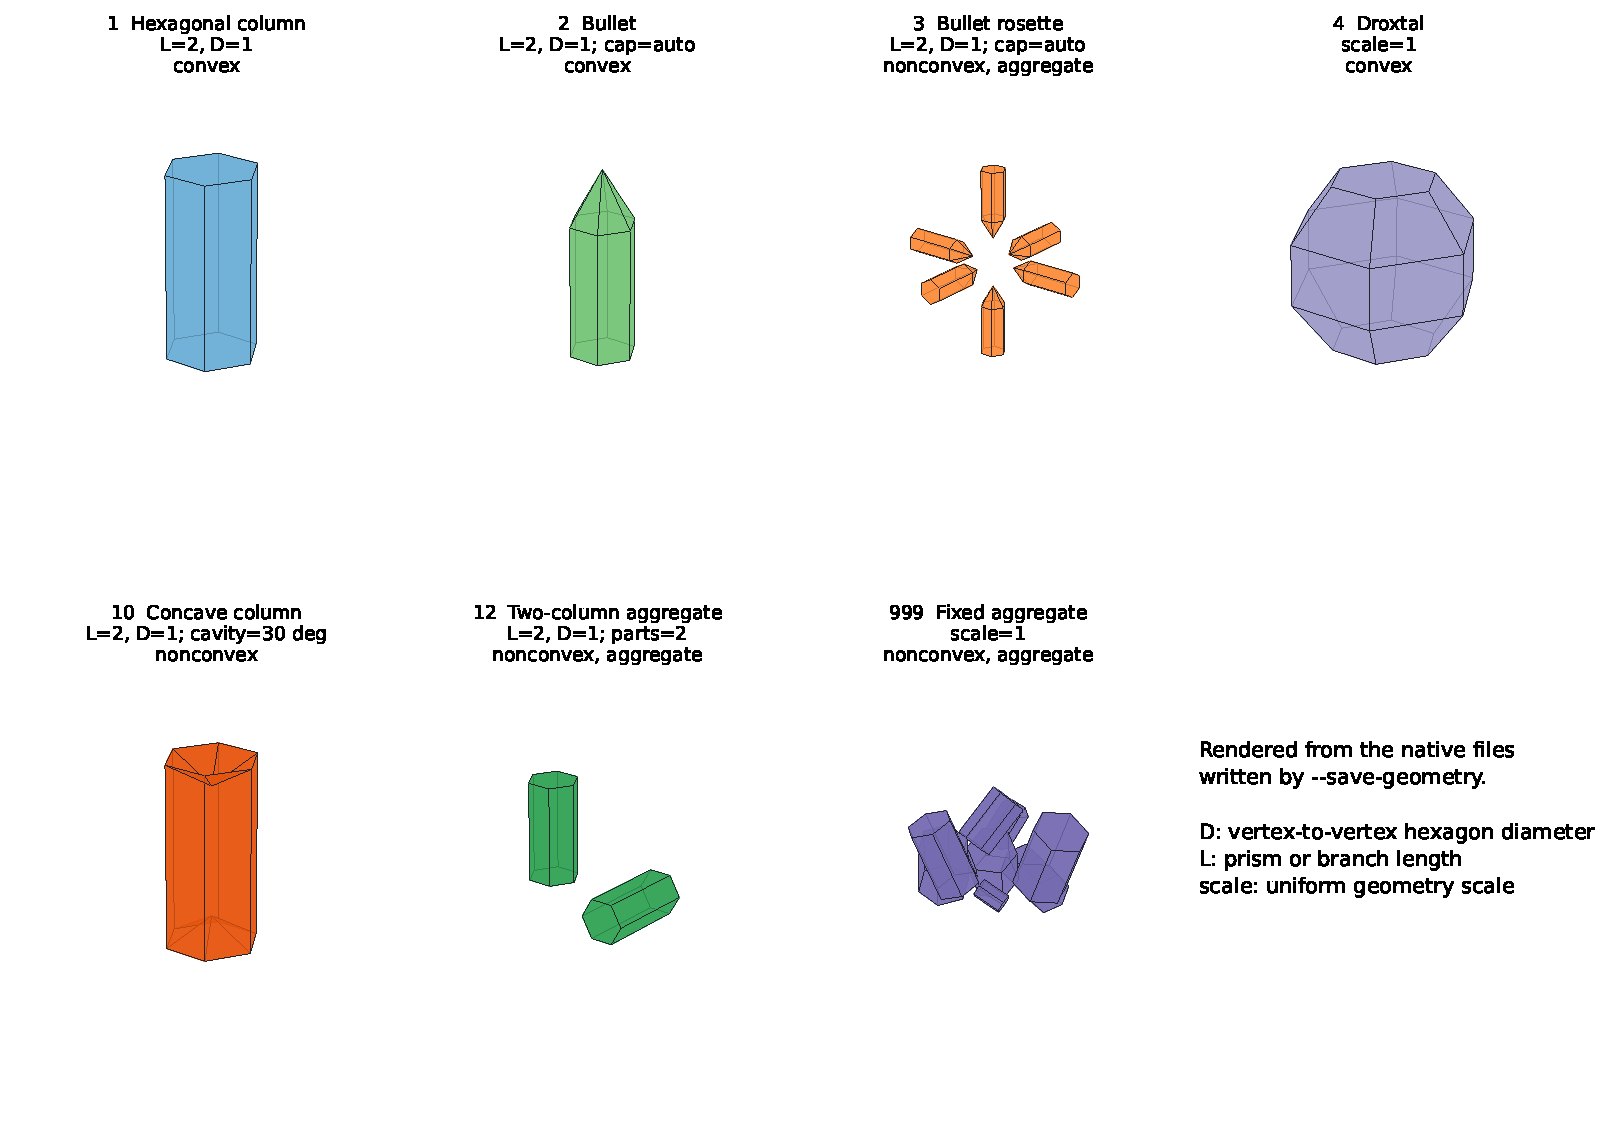
\includegraphics[width=0.98\linewidth]{manual_particle_gallery.pdf}
\caption{Geometries produced by the current built-in constructors. The images
are rendered from the native files in \texttt{examples/particles}, not from
separate drawing models.}
\label{fig:particle-gallery}
\end{figure}

\subsection{Native particle file and geometry export}

The native format starts with three nonempty header records:

\begin{Shaded}
\begin{Highlighting}[]
\NormalTok{CONCAVE}
\NormalTok{AGGREGATE [FACETS_PER_PART]}
\NormalTok{BETA_DOMAIN_DEG GAMMA_DOMAIN_DEG}
\NormalTok{}
\NormalTok{x0 y0 z0}
\NormalTok{x1 y1 z1}
\NormalTok{x2 y2 z2}
\NormalTok{}
\NormalTok{x0 y0 z0      \# next facet}
\NormalTok{...}
\end{Highlighting}
\end{Shaded}

\texttt{CONCAVE} is 0 or 1. \texttt{AGGREGATE} is 0 for one object, or
\texttt{1 FACETS\_PER\_PART} for equal-size aggregate components. The third
record gives the positive beta and gamma fundamental-domain widths. Blank
lines separate facets; each facet must have at least three finite,
non-collinear vertices. Full-line and inline comments begin with
\texttt{\#}. Each facet must be a simple planar convex polygon. Vertex order
defines its normal; every component must be a closed manifold with consistent
outward winding. A facet may contain at most 64 vertices and a particle at most
256 facets.

\texttt{-\/-save-geometry FILE} writes 17-digit coordinates. Loading validates
facet geometry, closed manifold topology, outward winding, and aggregate
metadata before tracing. A useful round-trip check is:

\begin{Shaded}
\begin{Highlighting}[]
\ExtensionTok{gpu/bin/mbs\_po\_gpu\_double\_fast} \AttributeTok{{-}{-}po} \AttributeTok{{-}p}\NormalTok{ 10 20 12 15 }\DataTypeTok{\textbackslash{}}
    \AttributeTok{{-}{-}save-geometry}\NormalTok{ concave.particle ...}
\ExtensionTok{gpu/bin/mbs\_po\_gpu\_double\_fast} \AttributeTok{{-}{-}po} \AttributeTok{{-}{-}pf}\NormalTok{ concave.particle ...}
\end{Highlighting}
\end{Shaded}

The export consists of \texttt{FILE} and \texttt{FILE.visibility}.  The
sidecar stores the two clipping-visibility flags of every facet and is loaded
automatically when it is present.  Keep both files together: coordinates
alone are insufficient for an exact round trip of concave built-in particles.
Geometry is not written automatically; request it explicitly with
\texttt{--save-geometry FILE} (alias \texttt{--save-particle}).

Equivalent-size scaling:

\begin{Shaded}
\begin{Highlighting}[]
\NormalTok{r\_eq = (3 V / (4*pi))\^{}(1/3)}
\NormalTok{k\_eq = 2*pi*r\_eq/lambda}
\NormalTok{scale = (k\_eq\_target * lambda / (2*pi)) / r\_eq\_original}
\end{Highlighting}
\end{Shaded}

\section{Orientation grids}\label{orientation-grids}

\begin{longtable}[]{@{}L{0.20\linewidth}L{0.14\linewidth}L{0.28\linewidth}L{0.28\linewidth}@{}}
\toprule\noalign{}
Mode & Arguments & Best use & Notes \\
\midrule\noalign{}
\endhead
\bottomrule\noalign{}
\endlastfoot
\texttt{-\/-oldauto} & \texttt{DIV} & Production regular grid & Grid
step follows diffraction-limited angular scale; common values are
\texttt{2}, \texttt{4}, \texttt{8}. \\
\texttt{-\/-random} & \texttt{Nb\ Ng} & Manual beta/gamma regular grid &
Uses symmetry-reduced beta/gamma domain unless overridden. \\
\texttt{-\/-fixed} & \texttt{BETA\ GAMMA} & Single-orientation debugging
& Angles are degrees. \\
\texttt{-\/-orientfile} & \texttt{FILE} & Reproducible custom
orientations & One beta/gamma pair in degrees per line. \\
\texttt{-\/-sobol} & \texttt{N} & Quasi-random orientation average &
Good convergence for broad scans. \\
\texttt{-\/-sobol\_seed} & \texttt{N\ S} & Seeded Sobol/Owen sequence &
Useful for repeatable convergence checks. \\
\texttt{-\/-sobol\_ring} & \texttt{Nb\ Ng} & Sobol beta with uniform
gamma rings & Hybrid orientation grid. \\
\texttt{-\/-so3\_quat} & \texttt{N} & Isotropic SO(3) average &
Hammersley on the symmetry quotient; laboratory alpha is integrated by
scattering phi. \\
\texttt{-\/-so3\_full\_quat} & \texttt{N} & Independent SO(3) audit &
Direct full-group Shoemake quaternions; particle symmetry is deliberately
ignored. \\
\texttt{-\/-hammersley} & \texttt{N} & Low-discrepancy orientations &
Debug/experimental. \\
\texttt{-\/-lattice} & \texttt{N} & Rank-1 lattice orientations &
Debug/experimental. \\
\texttt{-\/-lattice\_z} & \texttt{N\ Z} & Rank-1 lattice with explicit
generator & Debug/experimental. \\
\texttt{-\/-euler\_quad} & \texttt{Nb\ Ng} & Gauss in cos(beta),
periodic gamma & High-order quadrature. \\
\texttt{-\/-euler\_adapt} & \texttt{Nb\ NgMax} & Adaptive gamma count
per beta ring & Reduces work near beta poles. \\
\texttt{-\/-adaptive\_euler} & \texttt{EPS} & Converged regular Euler grid &
Refines \(N_\beta\) and \(N_\gamma\) separately, then together. \\
\texttt{-\/-adaptive} & \texttt{EPS} & Adaptive Sobol count only & Doubles
\(N\); it does not silently alter theta, phi, or reflection depth. \\
\texttt{-\/-auto} & \texttt{EPS} & Auto theta, phi, orientation count &
Keeps the requested reflection depth fixed. \\
\texttt{-\/-autofull} & \texttt{EPS} & Auto \texttt{n}, theta, phi,
orientations & Slower, more complete search. \\
\texttt{-\/-oldautofull} & \texttt{EPS} & Autofull with converged Euler
grid & Independently converges \(N_\beta\) and \(N_\gamma\). \\
\texttt{-\/-adaptive-config} & \texttt{FILE} & Reproducible adaptive
settings & Per-parameter minimum, maximum, and tolerance. \\
\end{longtable}

Orientation modifiers:

\begin{longtable}[]{@{}L{0.24\linewidth}L{0.22\linewidth}L{0.46\linewidth}@{}}
\toprule\noalign{}
Flag & Arguments & Description \\
\midrule\noalign{}
\endhead
\bottomrule\noalign{}
\endlastfoot
\texttt{-\/-ring\_points} & \texttt{N} & Points per diffraction ring for
oldauto estimates; default \texttt{3}. \\
\texttt{-\/-mirror\_gamma} & none & For a verified reflection-symmetric
particle, sample half the gamma range and restore the omitted Mueller
contribution with Stokes parity. Supported by \texttt{-\/-so3\_quat}. \\
\texttt{-\/-so3\_mirror\_audit} & none & With an even
\texttt{-\/-so3\_quat N}, explicitly trace nested reflected pairs for a
direct validation of \texttt{-\/-mirror\_gamma}. \\
\texttt{-\/-sym} & \texttt{Sb\ Sg} & Override symmetry domain: beta
range is \texttt{pi/Sb}, gamma range is \texttt{2*pi/Sg}. \\
\texttt{-\/-b} & \texttt{B1\ B2} & Manual beta range in degrees for
\texttt{-\/-random}. \\
\texttt{-\/-g} & \texttt{G1\ G2} & Manual gamma range in degrees for
\texttt{-\/-random}. \\
\texttt{-\/-maxorient} & \texttt{N} & Maximum orientations for adaptive
modes. \\
\texttt{-\/-max\_beta\_points} & \texttt{N} & Hard adaptive
\(N_\beta\) limit. \\
\texttt{-\/-max\_gamma\_points} & \texttt{N} & Hard adaptive
\(N_\gamma\) limit. \\
\texttt{-\/-chunk} & \texttt{N} & Orientation/gamma chunk size. \\
\texttt{-\/-coh\_orient} & none & Disabled legacy mode; cross-orientation
coherence is undefined without relative phases. \\
\texttt{-\/-pole} & none & Use one gamma value at beta poles. Best with
endpoint grids such as \texttt{-\/-oldauto}. \\
\texttt{-\/-owen\_avg} & \texttt{K} & Average \texttt{K} nested Owen
final seeds in \texttt{-\/-autofull}; default can be controlled by
environment. \\
\texttt{-\/-owen\_seeds} & \texttt{S...} & Explicit Owen seeds for
\texttt{-\/-autofull} final averaging. \\
\end{longtable}

\subsection{Symmetry-reduced SO(3) quadrature}

For an isotropic ensemble, the Haar measure in the Euler convention used by
the program is
\[
 dR \mathrel{\propto} \sin\beta\,d\beta\,d\gamma\,d\alpha.
\]
The production mode \texttt{-\/-so3-quaternion N} traces only the particle's
fundamental domain
$0\leq\beta\leq\beta_{\rm sym}$,
$0\leq\gamma<\gamma_{\rm sym}$.  For point $i=0,\ldots,N-1$,
\[
 u_i=\frac{i+1/2}{N},\qquad
 v_i=\operatorname{radical\_inverse}_2(i),
\]
\[
 \beta_i=\arccos\!\left[1-(1-\cos\beta_{\rm sym})u_i\right],\qquad
 \gamma_i=\gamma_{\rm sym}v_i,\qquad w_i=\frac1N.
\]
Thus the nodes are uniform in $\cos\beta$, not in $\beta$, and the normalized
weights satisfy $\sum_i w_i=1$.  The option \texttt{-\/-sym Sb Sg} overrides
the domain with $\beta_{\rm sym}=\pi/S_b$ and
$\gamma_{\rm sym}=2\pi/S_g$; use it only for an actual particle symmetry.

For a paired mirror validation, add \texttt{-\/-so3-mirror-audit} to an even
full count and put $K=N/2$. The audit evaluates the same formulas for
$i=0,\ldots,K-1$ with $u_i=(i+1/2)/K$ and
$\gamma_i=(\gamma_{\rm sym}/2)v_i$, then explicitly traces both
$(\beta_i,\gamma_i)$ and $(\beta_i,\gamma_{\rm sym}-\gamma_i)$ with weight
$1/N$. This layout nests exactly with a $K$-point
\texttt{-\/-mirror-gamma} run. Without the audit modifier the production
full-domain Hammersley sequence is unchanged.

With \texttt{-\/-mirror-gamma}, the sampled range becomes
$0\leq\gamma<\gamma_{\rm sym}/2$. The omitted half is restored before the
$\alpha$ quadrature as
\[
 M_{\rm full}(\theta,\phi)=\frac12\left[
 M_{\rm half}(\theta,\phi)+P M_{\rm half}(\theta,-\phi)P\right],\qquad
 P=\operatorname{diag}(1,1,-1,-1).
\]
This is valid only when the complete optical particle, including facet
visibility and material assignment, has the asserted reflection plane and the
selected PO tracer is numerically invariant under that reflection. The program
cannot prove this property from a particle file; validate every new particle
class and parameter regime against one full-gamma run. The value $N$ remains
the number of actually traced $\beta,\gamma$ orientations. For a strict paired
check, compare \texttt{-\/-so3-quaternion 4096 -\/-so3-mirror-audit} with
\texttt{-\/-so3-quaternion 2048 -\/-mirror-gamma}. Their base nodes are
identical, so the difference measures numerical mirror consistency rather than
two-sample Hammersley noise. Also check the ordinary full-domain sequence
against an independent dense result and inspect backscatter separately.

The remaining laboratory angle $\alpha$ is not retraced.  Rotation about the
incident beam is equivalent to changing scattering azimuth $\phi$, hence each
theta row is accumulated as
\[
 \overline{M}(\theta)=\frac{1}{N_\phi}
 \sum_{\phi} M(\theta,\phi)L(-\phi).
\]
Here $L$ is the Stokes reference-plane rotation whose $Q/U$ block contains
$\cos(2\phi)$ and $\sin(2\phi)$.  Multiplication is on the right because the
incident polarization basis changes.  At $\theta=0$ and $\theta=\pi$ the
azimuthal basis is singular; the implementation averages without $L$ and then
applies the exact forward/backward pole form.

This mode requires $N_\phi\geq2$.  A production command should combine it with
\texttt{-\/-scattering-diffraction-sampling Q} and
\texttt{-\/-latitude-phi-grid}.  The slower
\texttt{-\/-so3-full-quaternion N} retains direct full-group sampling as an
independent audit.  Its $N$ counts complete three-dimensional rotations,
whereas the production mode's $N$ counts traced beta/gamma orientations and
uses the phi grid for the alpha quadrature.

\section{Scattering grids}\label{scattering-grids}

\begin{longtable}[]{@{}L{0.24\linewidth}L{0.22\linewidth}L{0.46\linewidth}@{}}
\toprule\noalign{}
Flag & Arguments & Description \\
\midrule\noalign{}
\endhead
\bottomrule\noalign{}
\endlastfoot
\texttt{-\/-grid} & \texttt{T1\ T2\ Nphi\ Nth} & Uniform theta grid from
\texttt{T1} to \texttt{T2} degrees. Output has \texttt{Nth\ +\ 1} theta
rows. \\
\texttt{-\/-grid} & \texttt{R\ Nphi\ Nth} & Backscatter cone grid of
radius \texttt{R} degrees. \\
\texttt{-\/-tgrid} & \texttt{FILE} & Non-uniform theta grid in degrees,
one row per theta value. \\
\texttt{-\/-auto\_tgrid} & \texttt{EPS} & Adaptive theta grid by
bisection of measured full-Mueller interpolation error; no fixed halo
angles are used. \\
\texttt{-\/-auto\_phi} & none & Compatibility form of measured phi
convergence with tolerance \(0.02\). \\
\texttt{-\/-adaptive\_phi} & \texttt{EPS} & Converge \(N_\phi\) only. \\
\texttt{-\/-adaptive\_reflections} & \texttt{EPS} & Converge internal
reflection depth \(n\) only. \\
\texttt{-\/-nphi} & \texttt{N} & Override phi count. Highest priority
for phi. \\
\texttt{-\/-diffraction-limit-grid} & \texttt{FACTOR} & Derive uniform
theta and equatorial-phi steps from the diffraction estimate. \\
\texttt{-\/-latitude-phi-grid} & none & Reduce the phi count in
proportion to $\sin\theta$ away from the equator. \\
\texttt{-\/-max\_theta\_points} & \texttt{N} & Hard theta-point limit;
default 4097. \\
\texttt{-\/-max\_phi\_points} & \texttt{N} & Hard \(N_\phi\) limit;
default 2400. \\
\texttt{-\/-convergence\_passes} & \texttt{N} & Consecutive passing
refinements required; default 2. \\
\texttt{-\/-filter} & \texttt{DEG} & Restrict output to a backscattering
cone. Legacy/debug use. \\
\texttt{-\/-point} & none & Backscatter point mode. Legacy; avoid for
optimized regular-grid production. \\
\end{longtable}

\subsection{Diffraction-limit and latitude-phi grids}

For a PO \texttt{-\/-diffraction-grid DIV} run,
\texttt{-\/-diffraction-limit-grid FACTOR} derives the scattering grid from
the current particle maximum dimension $l_{\max}$ and wavelength $\lambda$:
\[
 \xi=\mathrm{FACTOR}\,0.69\frac{\lambda}{l_{\max}},\qquad
 N_\theta=\left\lceil\frac{\pi}{\xi}\right\rceil,
\]
\[
 N_{\phi,\mathrm{eq}}=
 \operatorname{round\_up}_6\!\left[
  \max\!\left(12,\left\lceil\frac{2\pi}{\xi}\right\rceil\right)
 \right].
\]
The output contains $N_\theta+1$ rows from zero to $\pi$.
\texttt{FACTOR=1} uses the estimate literally; \texttt{FACTOR=0.5}
approximately halves both angular steps, while a factor above one makes the
grid coarser. This is an a-priori resolution estimate, not an a-posteriori
accuracy guarantee. Validate a production factor against a finer value for
every required Mueller element.

With \texttt{-\/-latitude-phi-grid}, each theta row uses
\[
 N_\phi(\theta)=\min\!\left\{N_{\phi,\mathrm{eq}},
 \operatorname{round\_up}_6\!\left[
  \max\!\left(12,
   \left\lceil\frac{2\pi\sin\theta}{\xi}\right\rceil\right)
 \right]\right\}.
\]
Equatorial spacing is unchanged while redundant azimuth samples are removed
near the poles. Counts are rounded to a multiple of six, and a pole shares
its neighboring work group for stable basis handling. Accumulation still uses
the full rectangular $N_{\phi,\mathrm{eq}}$ output layout, so the file format
does not change.

The variable latitude grid supports both
\texttt{-\/-method po -\/-diffraction-grid DIV} and the symmetry-reduced
\texttt{-\/-so3-quaternion N} path, with one particle size per process.  For
SO(3), prefer \texttt{-\/-scattering-diffraction-sampling Q}; the unified
\texttt{-\/-diffraction-sampling Q} is itself a primary regular orientation
rule.  The diffraction-limit option conflicts with explicit
\texttt{-\/-nphi}; the latitude grid is not supported by a shared serial
multi-size trace. Run each size in its own process so $l_{\max}$ and the grid
are recomputed.

\begin{Shaded}
\begin{Highlighting}[]
\VariableTok{CUDA_VISIBLE_DEVICES}\OperatorTok{=}\NormalTok{0,1,2,3 }\DataTypeTok{\textbackslash{}}
\VariableTok{MBS_GPU_GROUPS}\OperatorTok{=}\NormalTok{1 }\VariableTok{MBS_GPU_MULTI_MAX}\OperatorTok{=}\NormalTok{4 }\DataTypeTok{\textbackslash{}}
\ExtensionTok{gpu/bin/mbs_po_gpu_double}\NormalTok{ ... }\AttributeTok{{-}{-}diffraction-limit-grid}\NormalTok{ 0.5 }\AttributeTok{{-}{-}latitude-phi-grid}
\end{Highlighting}
\end{Shaded}

Selection rules:

\begin{longtable}[]{@{}L{0.30\linewidth}L{0.64\linewidth}@{}}
\toprule\noalign{}
Quantity & Rule \\
\midrule\noalign{}
\endhead
\bottomrule\noalign{}
\endlastfoot
Theta grid & Exactly one of \texttt{-\/-tgrid}, \texttt{-\/-grid}, or
\texttt{-\/-auto\_tgrid}; unified auto modes treat an explicit grid as fixed. \\
Phi grid & Standalone adaptive phi selection and explicit
\texttt{-\/-nphi} are mutually exclusive. Unified auto modes treat explicit
\texttt{-\/-nphi} as fixed and tune the remaining dimensions. \\
\end{longtable}

\subsection{Unified convergence criterion}

For two approximations \(A\) and \(B\), phi, reflection, and Euler
candidate comparisons use the row error
\[
 e_{\mathrm{row}}=\max\!\left(
 \frac{|M^{A}_{11}-M^{B}_{11}|}
      {\max(|M^{A}_{11}|,|M^{B}_{11}|,\epsilon_0)},
 \max_{(i,j)\ne(1,1)}
 \frac{|R^{A}_{ij}-R^{B}_{ij}|}
      {\max(1,|R^{A}_{ij}|,|R^{B}_{ij}|)}
 \right),
 \qquad R_{ij}=\frac{M_{ij}}{M_{11}}.
\]
Here \(M_{ij}\) is a Mueller element, \(R_{ij}\) is its normalized
value, and \(\epsilon_0\) protects a vanishing \(M_{11}\).  The maximum
over theta rows is combined with the relative change of
\(\int M_{11}\,d\Omega\). Reflection-depth tests also include outgoing
energy. Theta convergence is different: it evaluates the actual Mueller row
at one-third and two-thirds of every interval against interpolation and checks
the same integrated \(M_{11}\). Sobol orientation convergence checks incoming
energy and all 16 Mueller elements on control-theta rows selected from the
actual scattering grid.

The parameters are not strictly independent. Reflection depth changes the
beam tree; phi changes the azimuth average used to expose theta structure;
and orientation sampling changes every averaged row. Therefore the joint
order is
\[
 n\longrightarrow N_\phi\longrightarrow
 \{\theta_j\}\longrightarrow N_{\mathrm{orient}}.
\]
The \texttt{-\/-auto} modes repeat the complete sequence on a common larger
pilot set until the pilot implied by the selected orientation count and all
selected values form a coupled fixed point. Regular Euler convergence
alternates \(N_\beta\) and \(N_\gamma\), then doubles both together. Reaching
any hard limit in phi, reflection, theta, Euler, or a unified mode is reported
as an error rather than accepted as convergence. Standalone
\texttt{-\/-adaptive-orientations} is exploratory: at its orientation cap it
warns and writes the best result; unified modes use strict orientation
convergence. The configured passing streak applies to phi, reflection, Euler,
and orientation searches, while theta uses interval refinement directly.
Every trial is written to
\texttt{<output>/<name>\_convergence.tsv}.

\subsection{Adaptive configuration file}

Use \texttt{-\/-adaptive-config FILE} to keep production convergence
settings outside a long command line. The documented template is
\texttt{configs/adaptive.example.conf}. It uses strict
\texttt{key = value} assignments and accepts inline comments after
\texttt{\#} or \texttt{;}.

The file defines separate minimum, maximum, and relative tolerance values for
reflection depth, laboratory alpha (internally \(N_\phi\)), theta points,
Sobol orientations, beta points, and gamma points. It also defines the number
of consecutive passing refinements and the pilot and sweep limits of the
coupled controller. A tolerance of \texttt{0.01} means one percent.

\begin{Shaded}
\begin{Highlighting}[]
\NormalTok{mbs_po --autofull 0.02 --adaptive-config configs/adaptive.example.conf ...}
\end{Highlighting}
\end{Shaded}

Per-parameter tolerances in the file replace the mode-wide \texttt{EPS}; a
missing tolerance inherits \texttt{EPS}. Explicit command-line
\texttt{-\/-max-*}, \texttt{-\/-max-reflections}, and
\texttt{-\/-convergence-passes} values override the file. Unknown keys,
duplicates, invalid ranges, non-power-of-two Sobol limits, and malformed lines
are rejected before the calculation, with the file line and a corrective hint.

\subsection{Why column symmetry does not divide Nphi}

The code uses the Euler convention
\[
 \mathbf{R}=R_z(\alpha)R_y(\beta)R_z(\gamma).
\]
The scattering-azimuth loop is the rotationally covariant implementation of
the laboratory-angle \(\alpha\) average, so \(N_\phi=N_\alpha\) in this
context. A hexagonal column has the body-axis symmetry
\(R_z(2\pi/6)\); it reduces the \(\gamma\) domain to
\(0\leq\gamma<\pi/3\). For \(\beta\ne0,\pi\), it does not make the tilted
particle invariant under a laboratory \(R_z(2\pi/6)\) rotation, hence
\(0\leq\alpha<2\pi\) is still required. An automatic division of
\(N_\phi\) by six would therefore be incorrect. The aliases
\texttt{-\/-alpha-points} and \texttt{-\/-adaptive-alpha} only clarify the
meaning of the existing phi controls; they do not enable an approximation.

For full angular integrals use \texttt{-\/-grid\ 0\ 180\ Nphi\ Nth}.
Endpoint rows are physical half-cells; they must not have zero weight.

\section{Beam and trace cutoffs}\label{beam-and-trace-cutoffs}

Cutoffs act at two different stages. Output-beam cutoffs discard a completed
ray branch before PO diffraction. Trace cutoffs stop an internal branch while
the reflection/refraction tree is being built. With reference values taken
from the current orientation, the three dimensionless tests are
\[
 j_b=\frac{\lVert J_b\rVert_F^2}{J_{\mathrm{ref}}^2},\qquad
 a_b=\frac{A_b}{A_{\mathrm{ref}}},\qquad
 i_b=j_ba_b.
\]
Here $J_b$ is the accumulated Jones matrix of branch $b$, $A_b$ is its
polygon area, and $i_b$ is a simple intensity-area importance estimate.
When several tests are enabled, rejection uses logical \emph{OR}: satisfying
any one smallness test removes the branch. Reason counters can therefore
overlap.

\subsection{Coherent presets}

\texttt{-\/-cutoff-profile MODE} configures all relative thresholds and the
small-fragment ratio together. It cannot be combined with an individual
cutoff or \texttt{-\/-beam-area-ratio}.

\begin{longtable}[]{@{}L{0.13\linewidth}L{0.17\linewidth}L{0.17\linewidth}L{0.17\linewidth}L{0.26\linewidth}@{}}
\toprule\noalign{}
Profile & Output $i_b$ & Trace $i_b$ & Area ratio & Intended use \\
\midrule\noalign{}
\endhead
\bottomrule\noalign{}
\endlastfoot
\texttt{off} & 0 & 0 & disabled & Reference and convergence runs; no
configurable cutoff approximation. \\
\texttt{safe} & $10^{-10}$ & $10^{-12}$ & $10^8$ & First production
candidate after comparison with \texttt{off}. \\
\texttt{balanced} & $10^{-8}$ & $10^{-10}$ & $10^5$ & Faster scans
after particle-class calibration. \\
\texttt{fast} & $10^{-6}$ & $10^{-8}$ & $10^3$ & Exploratory scans;
not a validation setting. \\
legacy default & 0 & $j_b=10^{-7}$ & 100 & Scale-invariant replacement of the historical weak-branch test when no profile
or individual cutoff is supplied. \\
\end{longtable}

The named \texttt{safe}, \texttt{balanced}, and \texttt{fast} presets enable the combined importance criterion, not separate
Jones and area OR thresholds. This avoids removing a large but weak branch or
a small but intense branch solely because one factor is small. The legacy
default additionally terminates a branch when its Jones norm is below
$10^{-7}$ of the strongest incident branch; this replaces the former
area-dependent threshold. Its area-ratio simplification remains at 100; use
\texttt{-\/-cutoff-profile off} when a genuinely uncut reference is required.
The profiles do not set \texttt{-\/-trace-max-beams}.  For unattended runs
on deeply concave particles, use a finite beam limit as a diagnostic guard:
strict profiles can still produce a very large tree for an isolated
orientation.  A nonzero ``Configured beam-limit hits'' counter means that the
result is incomplete; increase the limit or calibrate stronger cutoffs before
using that run as physical data.

\subsection{Individual controls}

\begin{longtable}[]{@{}L{0.31\linewidth}L{0.13\linewidth}L{0.50\linewidth}@{}}
\toprule\noalign{}
Flag & Range & Exact action \\
\midrule\noalign{}
\endhead
\bottomrule\noalign{}
\endlastfoot
\texttt{-\/-beam-cutoff EPS} & $[0,1]$ & Legacy shortcut setting both
output Jones and output area thresholds; a beam is rejected if either test
passes. \\
\texttt{-\/-beam-cutoff-jones EPS} & $[0,1]$ & Output test $j_b<\mathrm{EPS}$. \\
\texttt{-\/-beam-cutoff-area EPS} & $[0,1]$ & Output test $a_b<\mathrm{EPS}$. \\
\texttt{-\/-beam-cutoff-importance EPS} & $[0,1]$ & Output test
$i_b<\mathrm{EPS}$. \\
\texttt{-\/-trace-cutoff EPS} & $[0,1]$ & Legacy shortcut setting both
internal Jones and area thresholds; pruning uses OR. \\
\texttt{-\/-trace-cutoff-jones EPS} & $[0,1]$ & Internal test $j_b<\mathrm{EPS}$. \\
\texttt{-\/-trace-cutoff-area EPS} & $[0,1]$ & Internal test $a_b<\mathrm{EPS}$. \\
\texttt{-\/-trace-cutoff-importance EPS} & $[0,1]$ & Internal test
$i_b<\mathrm{EPS}$. \\
\texttt{-\/-beam-area-ratio R} & $R\ge1$ & After a nonconvex split,
replace two fragments by the larger one only when their area ratio is at
least $R$. \\
\texttt{-\/-trace-max-beams N} & $N\ge0$ & Hard per-orientation beam-tree
cap; 0 disables the configured cap. Reaching it aborts the calculation so an
incomplete orientation cannot enter the average. \\
\end{longtable}

If a legacy common shortcut and a corresponding specific Jones/area option
are supplied together, the specific value overrides that side and the
program prints a warning. A profile instead rejects such mixing as an input
error, so a command cannot silently become a partly modified preset.

Every completed run appends \texttt{OUTPUT BEAM CUTOFF REPORT} and
\texttt{TRACE CUTOFF REPORT} blocks to the log. They contain the selected
profile, effective thresholds, candidate/kept/rejected counts, overlapping
reason counts, fragment simplifications, configured-cap hits, and hard
internal tree-limit hits. Calibrate a profile by running the same geometry,
orientation set, $n$, theta grid, and $N_\phi$ with \texttt{off} and with
the candidate profile; compare all 16 $M_{ij}/M_{11}$, not only runtime or
the rejected-beam percentage.

\section{GPU and multi-GPU}\label{gpu-and-multi-gpu}

\subsection{CUDA backend}\label{cuda-backend}

\begin{longtable}[]{@{}L{0.30\linewidth}L{0.64\linewidth}@{}}
\toprule\noalign{}
Flag & Description \\
\midrule\noalign{}
\endhead
\bottomrule\noalign{}
\endlastfoot
\texttt{-\/-gpu} & Use CUDA diffraction backend. Optional in
\texttt{gpu/} binaries because they default to GPU. \\
\texttt{-\/-cpu} & Force CPU backend from a GPU-capable binary. \\
\texttt{-\/-fft} & Use cuFFT angular phi interpolation backend. Requires
GPU. The direct-phi compression factor is selected automatically. \\
\texttt{-\/-fft-factor N} & Enable FFT interpolation with an explicit
compression factor $1\le N\le64$. $N=1$ keeps the direct phi grid and is
useful as a same-backend reference. \\
\texttt{-\/-fft-tolerance EPS} & Enable a nested-grid error estimate and
one automatic refinement when the estimate exceeds $0<\mathrm{EPS}<1$. \\
\texttt{-\/-threads\ N} & OpenMP host worker threads. Also controls
tracing-side parallelism before GPU diffraction. \\
\end{longtable}

\subsection{FFT phi compression and error control}

Let $N_\phi$ be the requested output azimuth count and $f$ the compression
factor. The first CUDA pass evaluates approximately
\[
 N_{\phi,\mathrm{direct}}
 =\max\!\left(16,\left\lfloor\frac{N_\phi}{f}\right\rfloor\right)
\]
direct samples, then uses periodic Fourier zero-padding to reconstruct the
$N_\phi$ output grid. For $f=1$, $N_\phi<32$, or a factor that cannot
reduce the grid, the implementation uses the direct path. The speed gain is
therefore workload dependent and is bounded by the fraction of runtime spent
in phi-direction diffraction; tracing itself is not reduced.

\texttt{-\/-fft} asks the implementation to select $f$.
\texttt{-\/-fft-factor N} makes the requested compression explicit and has
priority over \texttt{MBS\_FFT\_PHI\_FACTOR}. Large factors are not an accuracy
promise: sharp azimuthal structure has high Fourier modes and can be smoothed
or aliased.

With \texttt{-\/-fft-tolerance EPS}, the code also evaluates a nested grid
with
\[
 N_{\phi,2}=\min(N_\phi,2N_{\phi,\mathrm{direct}}).
\]
It compares significant $M_{11}$ samples and all 16 Mueller elements using
an $M_{11}$-based scale. The reported estimate is
\[
 \widehat e=\max\!\left(
   \max_{M_{11}\ \mathrm{significant}}
     \frac{|M_{11}^{(1)}-M_{11}^{(2)}|}{|M_{11}^{(2)}|},
   \max_{i,j}\frac{|M_{ij}^{(1)}-M_{ij}^{(2)}|}
     {\max(|M_{11}^{(2)}|,10^{-3}M_{11,\max}^{(2)})}
 \right).
\]
If $\widehat e>\mathrm{EPS}$, the result reconstructed from the doubled direct grid
is retained. This is a one-step a-posteriori estimator, not a rigorous bound
and not an iterative convergence proof. It costs an additional diffraction
pass and temporarily holds coarse, refined, and output arrays. For a final
reference, omit all FFT flags or use \texttt{-\/-fft-factor 1}; for production,
first calibrate $f$ and EPS on representative sizes and particle shapes.

\begin{Shaded}
\begin{Highlighting}[]
\CommentTok{\# Explicit 4x compression, refine once when the estimate exceeds 1 percent}
\ExtensionTok{gpu/bin/mbs\_po\_gpu\_float\_fast}\NormalTok{ ... }\AttributeTok{{-}{-}fft-factor}\NormalTok{ 4 }\AttributeTok{{-}{-}fft-tolerance}\NormalTok{ 0.01}
\end{Highlighting}
\end{Shaded}

The final \texttt{FFT INTERPOLATION REPORT} records the requested and effective
factor, direct and output $N_\phi$, number of FFT-path and validation calls,
number of refined calls, and the worst nested-grid estimate. Factor 1 is
labelled as direct/no interpolation. The fused multi-
\texttt{k\_eq} FFT path does not perform this validation; when tolerance or
the diagnostic check is requested, the dispatcher uses a supported fallback
instead of silently skipping the check.

GPU runtime errors are fatal in the split GPU build. For debugging only:

For regular polygon phases, the CPU PO loop evaluates four adjacent theta
directions together with AVX2. The edge accumulation order is retained in
every vector lane. A small phase or an active near-singular denominator
selects the original stable scalar formula for that group. This selection is
automatic, has no command-line tolerance, and is enabled in the standard CPU
build. The temporary phase and sine/cosine arrays use a vertex-major,
theta-contiguous layout. Consequently, each AVX2 edge update loads four
adjacent theta values directly instead of gathering them from four rows. In
the representative absorbing concave benchmark this layout changed the median
time from 12.76~s to 11.37~s (1.12x) relative to the preceding vectorized
implementation, while the written Mueller table remained bit-identical.

\begin{Shaded}
\begin{Highlighting}[]
\VariableTok{MBS\_GPU\_ALLOW\_FALLBACK}\OperatorTok{=}\NormalTok{1 }\ExtensionTok{gpu/bin/mbs\_po\_gpu\_float\_fast}\NormalTok{ ...}
\end{Highlighting}
\end{Shaded}

\subsection{Why the GPU version is
faster}\label{why-the-gpu-version-is-faster}

The expensive PO part is the repeated evaluation of the same beam
aperture integral for many detector directions and many orientations.
The CPU traces rays and prepares compact beam records; the GPU then
evaluates diffraction and, in the fast paths, Mueller accumulation on a
large regular grid.

\begin{longtable}[]{@{}L{0.20\linewidth}L{0.22\linewidth}L{0.28\linewidth}L{0.20\linewidth}@{}}
\toprule\noalign{}
Work item & CPU path & GPU path & Parallel granularity \\
\midrule\noalign{}
\endhead
\bottomrule\noalign{}
\endlastfoot
Ray tracing through facets & OpenMP over orientations/gamma blocks &
Automatic CUDA ordering and conservative candidate filtering; exact
intersections and beam splitting remain CPU-side & Orientation/chunk level \\
Beam packing & CPU host code & CPU prepares \texttt{GpuBeam}/packed beam
buffers and copies to device & Beam records \\
Edge diffraction & Scalar/vector CPU loops & CUDA kernels in
\texttt{GpuDiffraction.cu} & Beam x theta x phi x orientation \\
Jones coherent sum & CPU arrays of complex 2x2 matrices & Atomic or
no-atomic device kernels & Grid cell and orientation \\
Jones to Mueller & CPU after Jones sum & Separate
\texttt{mueller\_batch\_kernel} or fused in diffraction kernel & Grid
cell \\
Multi-\texttt{k\_eq} scans & Repeat diffraction per size & Optional
fused multi-\texttt{k\_eq} CUDA pass & Size x beam x grid \\
FFT phi interpolation & CPU direct phi grid unless disabled & cuFFT
low-phi pass plus zero-padding reconstruction & Theta/orientation
batches \\
\end{longtable}

The main speedup comes from exposing a very large product of independent
operations:

\begin{Shaded}
\begin{Highlighting}[]
\NormalTok{Nwork \textasciitilde{}= Norient * Nbeams\_per\_orientation * Ntheta * Nphi}
\end{Highlighting}
\end{Shaded}

Each beam/direction contribution is mostly independent until the
coherent Jones sum. That makes the diffraction stage a good CUDA
workload: many threads do the same edge-integral arithmetic over
different \texttt{(orientation,\ beam,\ theta,\ phi)} combinations.

\subsection{Atomic and no-atomic GPU
accumulation}\label{atomic-and-no-atomic-gpu-accumulation}

There are two families of CUDA accumulation paths in
\texttt{src/cuda/GpuDiffraction.cu}.

\begin{longtable}[]{@{}L{0.20\linewidth}L{0.22\linewidth}L{0.28\linewidth}L{0.20\linewidth}@{}}
\toprule\noalign{}
Mode & Main kernels & How accumulation works & When useful \\
\midrule\noalign{}
\endhead
\bottomrule\noalign{}
\endlastfoot
Atomic Jones accumulation & \nolinkurl{diffraction_kernel} & Each thread
computes one beam/grid contribution and uses \texttt{atomicAdd} into the
complex Jones buffer. Afterwards \nolinkurl{mueller_batch_kernel}
converts the summed Jones matrix to Mueller. & General fallback,
supports more combinations such as no-shadow output. \\
No-atomic grid kernels & \nolinkurl{diffraction_grid_kernel} & Work is
reorganized so a thread owns a grid/output slot and loops over beams,
avoiding multiple writers to the same Jones cell. & Full-only output
when memory/layout allows it. \\
Fused Mueller kernels & \nolinkurl{diffraction_grid_mueller_kernel},
\nolinkurl{diffraction_grid_mueller_full_kernel},
\nolinkurl{*_full8_kernel}, \nolinkurl{*_mixed8_kernel} & The kernel
computes coherent Jones locally for an output slot and immediately
converts/adds Mueller, avoiding large intermediate Jones buffers. & Fast
production path for full-only GPU runs. \\
Staged orientation Mueller &
\nolinkurl{diffraction_grid_mueller_orient_kernel} +
\nolinkurl{reduce_mueller_orient_kernel} & First writes per-orientation
Mueller, then reduces orientations. & Reduces contention and gives a
deterministic reduction shape for large orientation batches. \\
Multi-\texttt{k\_eq} fused &
\nolinkurl{diffraction_grid_mueller_multik_kernel} & Computes several
nearby equivalent sizes from one packed beam batch. & Shared-batch
\texttt{-\/-multikeq} scans. \\
\end{longtable}

In the atomic path the atomics are on the real and imaginary components
of the 2x2 Jones matrix:

\begin{Shaded}
\begin{Highlighting}[]
\NormalTok{J00.re, J00.im, J01.re, J01.im,}
\NormalTok{J10.re, J10.im, J11.re, J11.im}
\end{Highlighting}
\end{Shaded}

For \texttt{\_noshadow} output the same set of atomics is also applied
to the no-shadow Jones buffer. This is correct for coherent PO because
beams must be summed as Jones amplitudes before conversion to Mueller.
The cost is contention when many beams hit the same detector cell.

The no-atomic/fused paths avoid that contention by changing ownership:
one CUDA thread or thread group owns an output grid element and
accumulates the beams for that element in registers/local variables.
This is often faster for full Mueller output because it reduces
global-memory atomics and may skip the large intermediate Jones buffer.
The tradeoff is that these paths are more specialized and may be
disabled for diagnostic modes that require extra outputs.

Useful controls:

\begin{longtable}[]{@{}L{0.30\linewidth}L{0.64\linewidth}@{}}
\toprule\noalign{}
Environment variable & Effect \\
\midrule\noalign{}
\endhead
\bottomrule\noalign{}
\endlastfoot
\texttt{MBS\_GPU\_NO\_ATOMICS=1} & Force no-atomic path when
supported. \\
\texttt{MBS\_GPU\_NO\_ATOMICS=0} & Force atomic path for
comparison/debugging. \\
\texttt{MBS\_GPU\_FUSED\_MUELLER=1} & Prefer fused
diffraction-to-Mueller kernels when no-atomic mode is active. \\
\texttt{MBS\_GPU\_STAGE\_MUELLER=1} & Use staged per-orientation Mueller
plus reduction where supported. \\
\texttt{MBS\_GPU\_NO\_VERTEX\_CACHE=1} & Disable cached/packed vertex
path for debugging. \\
\texttt{MBS\_GPU\_COMPACT\_BEAMS=0} & Disable compact packing for beams
with at most 8 vertices and use the general layout for diagnostics. \\
\nolinkurl{MBS_GPU_COMPACT_BEAM4_SPLIT=0} & Disable separate four-vertex
records for triangles/quadrilaterals and use the previous eight-vertex
compact layout. \\
\texttt{MBS\_GPU\_WARP\_BEAMS=0/1} & Override automatic reduction: one
thread per output (0) or one warp per output (1). \\
\texttt{MBS\_GPU\_WARP\_GRID\_3D=0} & Disable the 3D-grid specialization
when warp reduction is active. \\
\texttt{MBS\_GPU\_THREAD\_GRID\_3D=0/1} & Override the tiled 3D-grid
layout for the consumer thread path. Automatic mode uses it with a
64-thread block when edge padding is at most 15\%. \\
\texttt{MBS\_GPU\_TIMING=1} & Print GPU timing breakdown for
count/pack/copy/kernels/d2h/add. \\
\texttt{MBS\_GPU\_BLOCK=N} & Override CUDA block size for kernel
tuning. \\
\end{longtable}

By default CUDA uses its reported FP32:FP64 throughput ratio. A ratio of 16
or greater selects one thread per output; lower ratios retain warp reduction.
The former was 2--11\% faster on an RTX 3080 Ti across the tested convex,
concave, FP32, FP64, and 8--20-reflection cases. V100/A100-class GPUs retain
the warp path. With the default 64-thread block the consumer path also uses
a $16\,\theta\times4\,\phi$ tiled grid when incomplete edge tiles add no more
than 15\% work. This removed two integer divisions per output thread and
changed wall time by 0--11\% in validation. \texttt{MBS\_GPU\_TIMING=1}
reports \texttt{reduction=thread|warp} and \texttt{layout=3d|flat}.

For the compact thread path, automatic packing separates polygons with at most
four vertices from polygons with five to eight vertices. Triangles and
quadrilaterals use compile-time loop lengths when every compact polygon has at
least three vertices. Packing uses one stable bucket pass instead of scanning
the beam list once per vertex count. On the RTX 3080 Ti concave absorbing probe
this reduced summed FP32 CUDA-kernel time by about 4\% and complete GPU
diffraction time by about 3\%; the short end-to-end run improved by about
2--3\% because CPU tracing was unchanged. FP64 was neutral in the kernel and
still benefited from reduced packing and transfer work. The release gate
compares this path with \texttt{MBS\_GPU\_COMPACT\_BEAM4\_SPLIT=0} in both
precision profiles.

\subsection{Automatic CUDA tracing profile}

The CUDA PO backend automatically enables batched facet ordering and
conservative projected candidate filtering. The same mode can be requested
explicitly with \nolinkurl{--gpu-trace-prefilter}; use
\nolinkurl{--no-gpu-trace-prefilter} for an A/B reference. This is not an
approximate beam tracer: exact intersection polygons, topology decisions,
Fresnel splitting, and child-beam construction remain on the CPU.

The validated automatic profile uses exact CUDA topological ordering, an
ordering cache, conservative skip flags for 25--256 candidates, cached facet
geometry, 64 threads for the large-list kernel, and one nonblocking CUDA stream
per OpenMP worker. The per-worker batch is
\(
  \max(64,\lceil512/N_{\mathrm{workers}}\rceil)
\),
which avoids the CUDA-stack exhaustion observed with oversized fixed batches.
If this initial batch still exhausts kernel-stack backing, the code recursively
splits it and remembers the reduced process-wide limit for all later batches
and orientations.
When trace-limit retries are enabled, worker copies also share the largest
successful retry beam limit. Later orientations skip the known-insufficient
first pass, but retry levels are still counted from the original configured
limit, so the retry ceiling is unchanged. On a 32-orientation nonconvex test,
this changed 11.12 s to 8.00 s and reduced full retries from 30 to 7.
Nonblocking per-worker streams changed a 256-orientation run from 61.39 s to
42.26 s. Output tables and integral files were byte-identical in both A/B
checks.
Independent processes on the same physical GPU serialize only the heavy trace
batch through a lock keyed by the PCI address. OpenMP workers within one
process retain independent streams and overlap. This default prevents combined
CUDA kernel-stack reservations from exhausting device memory and does not
serialize diffraction kernels.
On a deeply nonconvex production orientation this reduced wall time from
7.93 s to 0.98 s (8.09 times); on a smaller representative case the gain was
about 1.08 times. The benefit therefore depends strongly on trace complexity.

Expert controls are provided for reproducible profiling; their defaults form
the automatic profile:

\begin{longtable}[]{@{}L{0.38\linewidth}L{0.18\linewidth}L{0.36\linewidth}@{}}
\toprule\noalign{}
Variable & Default & Meaning \\
\midrule\noalign{}
\endhead
\bottomrule\noalign{}
\endlastfoot
\nolinkurl{MBS_GPU_TRACE_OPENMP} & 1 & Allow CUDA tracing from OpenMP workers. \\
\nolinkurl{MBS_GPU_TRACE_BATCH_BEAMS} & automatic & Override the initial per-worker batch; after OOM the process lowers and remembers the limit. \\
\nolinkurl{MBS_GPU_TRACE_FULL_SORT} & 1 & Exact CUDA topological ordering. \\
\nolinkurl{MBS_GPU_TRACE_SORT_CACHE} & 1 & Reuse exact ordering for identical keys. \\
\nolinkurl{MBS_GPU_TRACE_LARGE_SKIP_FLAGS} & 1 & Conservative projected skip flags. \\
\nolinkurl{MBS_GPU_TRACE_LARGE_THREADS} & 64 & Large-list block size (64, 128, or 256). \\
\nolinkurl{MBS_GPU_TRACE_CACHE_FACETS} & 1 & Retain packed facet geometry per worker. \\
\nolinkurl{MBS_GPU_TRACE_MIN_CANDIDATES} & 1024 & Minimum batch candidate count sent to CUDA. \\
\nolinkurl{MBS_GPU_TRACE_NONBLOCKING_STREAM} & 1 & Per-worker nonblocking streams; set 0 only for serialization diagnostics. \\
\nolinkurl{MBS_GPU_TRACE_PROCESS_LOCK} & 1 & Serialize heavy trace batches across independent processes on one physical GPU. \\
\nolinkurl{MBS_GPU_TRACE_PREFILTER_FIRST} & 0 & Diagnostic projected filtering before sorting. \\
\nolinkurl{MBS_GPU_TRACE_MARGIN} & automatic & Override the conservative projection margin. \\
\nolinkurl{MBS_GPU_TRACE_TIMING} & 0 & Print transfer and kernel timings. \\
\nolinkurl{MBS_GPU_TRACE_VERIFY_SORT} & 0 & Compare CUDA ordering and skip flags with CPU. \\
\end{longtable}

The verification mode reported zero ordering and skip-flag mismatches in the
production regression. Because a different but equivalent facet traversal can
change floating-point summation order, validate sensitive runs against
\nolinkurl{--no-gpu-trace-prefilter}; the release gate performs this A/B check.

For a variable latitude-phi grid, \texttt{MBS\_GPU\_GROUPS=1} enables a
dedicated exact scheduler. Independent theta-row work groups are assigned
dynamically to visible GPUs. Orientation tracing and prepared beams remain
shared in host memory, while each device owns one CUDA workspace. Packed
beams, weights, and offsets are uploaded once per orientation chunk per
device and reused for subsequent theta groups handled by that worker.

Use \nolinkurl{CUDA_VISIBLE_DEVICES} to select devices. Use
\nolinkurl{MBS_GPU_MULTI=N} or \nolinkurl{MBS_GPU_MULTI_MAX=N} to limit the
number of workers; \nolinkurl{MBS_GPU_MULTI=0} leaves one GPU. The scheduler
requires direct CUDA diffraction; FFT interpolation and theta-zone beam
filtering retain the existing path. Speedup need not be linear because CPU
tracing, packing, PCIe transfers, final reduction, and theta-group imbalance
remain in wall time.

\subsection{Multi-size scans}\label{multi-size-scans}

\begin{longtable}[]{@{}L{0.24\linewidth}L{0.22\linewidth}L{0.46\linewidth}@{}}
\toprule\noalign{}
Flag & Arguments & Description \\
\midrule\noalign{}
\endhead
\bottomrule\noalign{}
\endlastfoot
\texttt{-\/-multigrid} & \texttt{Dmin\ Dmax\ N} & Log-spaced scan in
absolute maximum particle dimension; each value uses
\(x=\pi D_{\max}/\lambda\), independent of the source size. \\
\texttt{-\/-multikeq} & \texttt{Kmin\ Kmax\ N} & Log-spaced scan in
equivalent size parameter. \\
\texttt{-\/-multikeq\_list} & \texttt{FILE} & Exact list of
\texttt{k\_eq} values, one per line. \\
\texttt{-\/-multigrid\_parallel} & \texttt{N} & Run scan points as child
processes; \texttt{0} means auto. \\
\texttt{-\/-multigrid\_threads} & \texttt{N} & OpenMP threads per child
process. \\
\texttt{-\/-gpu\_devices} & \texttt{LIST} & Comma-separated CUDA device
list, for example \texttt{0,1,2,3,4}. \\
\nolinkurl{--multikeq_shared_batches} & none & Batch nearby
\texttt{k\_eq} values per GPU child and reuse tracing from the largest
value in the batch. \\
\texttt{-\/-multikeq\_batch\_ratio} & \texttt{R} & Maximum
\texttt{kmax/kmin} inside one shared batch; default \texttt{1.05}. \\
\end{longtable}

Exact multi-GPU scan, one process per active GPU slot:

\begin{Shaded}
\begin{Highlighting}[]
\ExtensionTok{gpu/bin/mbs\_po\_gpu\_float\_fast} \AttributeTok{{-}{-}po} \AttributeTok{{-}{-}pf}\NormalTok{ particle.dat }\DataTypeTok{\textbackslash{}}
    \AttributeTok{{-}{-}multikeq\_list}\NormalTok{ keq.txt }\AttributeTok{{-}{-}ri}\NormalTok{ 1.6 0.002 }\AttributeTok{{-}w}\NormalTok{ 1.064 }\AttributeTok{{-}n}\NormalTok{ 12 }\DataTypeTok{\textbackslash{}}
    \AttributeTok{{-}{-}oldauto}\NormalTok{ 2 }\AttributeTok{{-}{-}grid}\NormalTok{ 0 180 600 180 }\AttributeTok{{-}{-}fft} \AttributeTok{{-}{-}close} \DataTypeTok{\textbackslash{}}
    \AttributeTok{{-}{-}multigrid\_parallel}\NormalTok{ 0 }\AttributeTok{{-}{-}multigrid\_threads}\NormalTok{ 16 }\AttributeTok{{-}{-}gpu\_devices}\NormalTok{ 0,1,2,3,4 }\DataTypeTok{\textbackslash{}}
    \AttributeTok{{-}o}\NormalTok{ scan\_exact}
\end{Highlighting}
\end{Shaded}

Shared-batch scan:

\begin{Shaded}
\begin{Highlighting}[]
\ExtensionTok{gpu/bin/mbs\_po\_gpu\_float\_fast} \AttributeTok{{-}{-}po} \AttributeTok{{-}{-}pf}\NormalTok{ particle.dat }\DataTypeTok{\textbackslash{}}
    \AttributeTok{{-}{-}multikeq\_list}\NormalTok{ keq.txt }\AttributeTok{{-}{-}ri}\NormalTok{ 1.6 0.002 }\AttributeTok{{-}w}\NormalTok{ 1.064 }\AttributeTok{{-}n}\NormalTok{ 12 }\DataTypeTok{\textbackslash{}}
    \AttributeTok{{-}{-}oldauto}\NormalTok{ 2 }\AttributeTok{{-}{-}grid}\NormalTok{ 0 180 600 180 }\AttributeTok{{-}{-}fft} \AttributeTok{{-}{-}close} \DataTypeTok{\textbackslash{}}
    \AttributeTok{{-}{-}multigrid\_parallel}\NormalTok{ 0 }\AttributeTok{{-}{-}multigrid\_threads}\NormalTok{ 16 }\AttributeTok{{-}{-}gpu\_devices}\NormalTok{ 0,1,2,3,4 }\DataTypeTok{\textbackslash{}}
    \AttributeTok{{-}{-}multikeq\_shared\_batches} \AttributeTok{{-}{-}multikeq\_batch\_ratio}\NormalTok{ 1.05 }\DataTypeTok{\textbackslash{}}
    \AttributeTok{{-}o}\NormalTok{ scan\_shared}
\end{Highlighting}
\end{Shaded}

Experimental fused multi-\texttt{k\_eq} GPU diffraction:

\begin{Shaded}
\begin{Highlighting}[]
\VariableTok{MBS\_GPU\_MULTI\_K\_FULL}\OperatorTok{=}\NormalTok{1 }\ExtensionTok{gpu/bin/mbs\_po\_gpu\_float\_fast}\NormalTok{ ...}
\end{Highlighting}
\end{Shaded}

Use tighter \texttt{-\/-multikeq\_batch\_ratio} for accuracy; use exact
mode when each size must have its own oldauto reference grid.

\section{All flags}\label{all-flags}

\subsection{Method, particle, and physical
parameters}\label{method-particle-and-physical-parameters}

\begin{longtable}[]{@{}L{0.24\linewidth}L{0.22\linewidth}L{0.46\linewidth}@{}}
\toprule\noalign{}
Flag & Arguments & Description \\
\midrule\noalign{}
\endhead
\bottomrule\noalign{}
\endlastfoot
\texttt{-\/-po} & none & Physical Optics mode. \\
\texttt{-\/-go} & none & Geometrical Optics mode. \\
\texttt{-p} & \texttt{TYPE\ L\ D\ {[}extra{]}} & Built-in particle. \\
\texttt{-\/-pf} & \texttt{FILE} & Particle from file. \\
\texttt{-\/-save-geometry} & \texttt{FILE} & Save the effective native
particle and continue; alias \texttt{-\/-save-particle}. \\
\texttt{-\/-rs} & \texttt{SIZE} & Resize file particle by Dmax. \\
\texttt{-\/-k\_eq} & \texttt{X} & Resize by equivalent size
parameter. \\
\texttt{-\/-ri} & \texttt{Re\ Im} & Refractive index. \\
\texttt{-w} & \texttt{LAMBDA} & Wavelength in micrometers. \\
\texttt{-n} & \texttt{N} & Maximum internal reflections/refractions. \\
\texttt{-\/-abs} & none & Enable absorption accounting. Also enabled
automatically for nonzero \texttt{Im(ri)}. \\
\texttt{-\/-abs\_points} & \texttt{N} or \texttt{all} & Absorption
sampling: center point or all polygon vertices. \\
\end{longtable}

\subsection{Orientation flags}\label{orientation-flags}

\begin{longtable}[]{@{}L{0.24\linewidth}L{0.22\linewidth}L{0.46\linewidth}@{}}
\toprule\noalign{}
Flag & Arguments & Description \\
\midrule\noalign{}
\endhead
\bottomrule\noalign{}
\endlastfoot
\texttt{-\/-fixed} & \texttt{BETA\ GAMMA} & Single orientation in
degrees. \\
\texttt{-\/-random} & \texttt{Nb\ Ng} & Regular beta/gamma grid. \\
\texttt{-\/-sobol} & \texttt{N} & Sobol orientations. \\
\texttt{-\/-so3\_quat} & \texttt{N} & Symmetry-reduced SO(3); alpha is
integrated by scattering phi. \\
\texttt{-\/-so3\_full\_quat} & \texttt{N} & Direct full-SO(3) quaternion
audit. \\
\texttt{-\/-sobol\_seed} & \texttt{N\ S} & Sobol with explicit Owen
seed. \\
\texttt{-\/-sobol\_ring} & \texttt{Nb\ Ng} & Sobol beta with gamma
rings. \\
\texttt{-\/-hammersley} & \texttt{N} & Hammersley orientation set. \\
\texttt{-\/-lattice} & \texttt{N} & Rank-1 lattice orientation set. \\
\texttt{-\/-lattice\_z} & \texttt{N\ Z} & Rank-1 lattice with explicit
generator. \\
\texttt{-\/-euler\_quad} & \texttt{Nb\ Ng} & Gauss beta x periodic gamma
quadrature. \\
\texttt{-\/-euler\_adapt} & \texttt{Nb\ NgMax} & Gauss beta with
adaptive gamma count. \\
\texttt{-\/-adaptive\_euler} & \texttt{EPS} & Independently converge
\(N_\beta\) and \(N_\gamma\), then verify them jointly. \\
\texttt{-\/-montecarlo} & \texttt{N} & Pseudo-random Monte Carlo
orientations. \\
\texttt{-\/-adaptive} & \texttt{EPS} & Adaptive Sobol orientation count
only. \\
\texttt{-\/-auto} & \texttt{EPS} & Auto theta, phi, and orientation
count. \\
\texttt{-\/-autofull} & \texttt{EPS} & Auto \texttt{n}, theta, phi, and
orientations. \\
\texttt{-\/-oldautofull} & \texttt{EPS} & Autofull search with a
converged regular Euler final grid. \\
\texttt{-\/-adaptive-config} & \texttt{FILE} & Load per-parameter
adaptive ranges and tolerances. \\
\texttt{-\/-owen\_avg} & \texttt{K} & Average final Owen seeds. \\
\texttt{-\/-owen\_seeds} & \texttt{S...} & Explicit final Owen seeds. \\
\texttt{-\/-oldauto} & \texttt{DIV} & Physics-based regular grid. \\
\texttt{-\/-ring\_points} & \texttt{N} & Points per diffraction ring
estimate. \\
\texttt{-\/-mirror\_gamma} & none & Use mirrored half gamma domain. \\
\texttt{-\/-orientfile} & \texttt{FILE} & Load beta/gamma orientations
in degrees from file. \\
\texttt{-\/-b} & \texttt{B1\ B2} & Beta range for
\texttt{-\/-random}. \\
\texttt{-\/-g} & \texttt{G1\ G2} & Gamma range for
\texttt{-\/-random}. \\
\texttt{-\/-maxorient} & \texttt{N} & Maximum adaptive orientation
count. \\
\texttt{-\/-max\_beta\_points} & \texttt{N} & Maximum adaptive
\(N_\beta\). \\
\texttt{-\/-max\_gamma\_points} & \texttt{N} & Maximum adaptive
\(N_\gamma\). \\
\texttt{-\/-chunk} & \texttt{N} & Chunk size for orientation/gamma
processing. \\
\texttt{-\/-coh\_orient} & none & Disabled legacy mode; do not use. \\
\texttt{-\/-pole} & none & Exact beta-pole gamma shortcut. \\
\texttt{-\/-sym} & \texttt{Sb\ Sg} & Override particle symmetry. \\
\end{longtable}

\subsection{Scattering grid and acceleration
flags}\label{scattering-grid-and-acceleration-flags}

\begin{longtable}[]{@{}L{0.24\linewidth}L{0.22\linewidth}L{0.46\linewidth}@{}}
\toprule\noalign{}
Flag & Arguments & Description \\
\midrule\noalign{}
\endhead
\bottomrule\noalign{}
\endlastfoot
\texttt{-\/-grid} & \texttt{T1\ T2\ Nphi\ Nth} & Uniform theta range. \\
\texttt{-\/-grid} & \texttt{R\ Nphi\ Nth} & Backscatter cone. \\
\texttt{-\/-tgrid} & \texttt{FILE} & Non-uniform theta grid. \\
\texttt{-\/-auto\_tgrid} & \texttt{EPS} & Adaptive theta grid. \\
\texttt{-\/-auto\_phi} & none & Measured phi convergence at tolerance
0.02. \\
\texttt{-\/-adaptive\_phi} & \texttt{EPS} & Converge \(N_\phi\) only. \\
\texttt{-\/-adaptive\_reflections} & \texttt{EPS} & Converge \(n\) only. \\
\texttt{-\/-nphi} & \texttt{N} & Override phi count. \\
\texttt{-\/-diffraction-limit-grid} & \texttt{FACTOR} & Set theta and
equatorial-phi steps to $\mathrm{FACTOR}\,0.69\lambda/l_{\max}$. \\
\texttt{-\/-latitude-phi-grid} & none & Use a row-dependent phi count
proportional to $\sin\theta$. \\
\texttt{-\/-max\_theta\_points} & \texttt{N} & Adaptive theta limit. \\
\texttt{-\/-max\_phi\_points} & \texttt{N} & Adaptive phi limit. \\
\texttt{-\/-convergence\_passes} & \texttt{N} & Required passing streak. \\
\texttt{-\/-threads} & \texttt{N} & OpenMP worker threads. \\
\texttt{-\/-gpu} & none & CUDA backend. \\
\texttt{-\/-cpu} & none & Force CPU backend in GPU build. \\
\texttt{-\/-fft} & none & cuFFT phi interpolation with automatic
compression. \\
\texttt{-\/-fft-factor} & \texttt{N} & Explicit direct/output phi
compression, $1\ldots64$; also enables FFT. \\
\texttt{-\/-fft-tolerance} & \texttt{EPS} & Nested-grid estimate in
$0<\mathrm{EPS}<1$ with one doubled-direct-grid refinement. \\
\texttt{-\/-cutoff-profile} & \texttt{MODE} & Complete preset:
\texttt{off}, \texttt{safe}, \texttt{balanced}, or \texttt{fast}. \\
\texttt{-\/-beam-cutoff} & \texttt{EPS} & Legacy output shortcut; reject
when relative Jones OR area is below EPS. \\
\texttt{-\/-beam-cutoff-jones} & \texttt{EPS} & Output cutoff by relative
squared Jones magnitude. \\
\texttt{-\/-beam-cutoff-area} & \texttt{EPS} & Output cutoff by relative
beam area. \\
\texttt{-\/-beam-cutoff-importance} & \texttt{EPS} & Output cutoff by
relative Jones intensity times area. \\
\texttt{-\/-trace-cutoff} & \texttt{EPS} & Legacy internal shortcut;
prune when relative Jones OR area is below EPS. \\
\texttt{-\/-trace-cutoff-jones} & \texttt{EPS} & Prune trace tree by
relative squared Jones magnitude. \\
\texttt{-\/-trace-cutoff-area} & \texttt{EPS} & Prune trace tree by
relative area. \\
\texttt{-\/-trace-cutoff-importance} & \texttt{EPS} & Prune trace tree
by relative Jones intensity times area. \\
\texttt{-\/-trace-max-beams} & \texttt{N} & Hard per-orientation beam-tree
cap; \texttt{0} disables it and reaching it aborts the calculation. \\
\nolinkurl{--gpu-trace-prefilter} & none & Explicitly enable the automatic
batched CUDA ordering and candidate-filtering profile. \\
\nolinkurl{--no-gpu-trace-prefilter} & none & Disable automatic CUDA tracing
for a reference comparison. \\
\texttt{-\/-trace\_prefilter} & none & Enable CPU projected-AABB
prefilter. \\
\texttt{-\/-no\_trace\_prefilter} & none & Disable CPU projected-AABB
prefilter. \\
\nolinkurl{--trace_prefilter_margin} & \texttt{M} & AABB prefilter
margin. \\
\texttt{-\/-trace\_prefilter\_stats} & none & Print prefilter
counters. \\
\texttt{-r}, \texttt{-\/-beam-area-ratio} & \texttt{RATIO} & Small-fragment
area ratio, at least 1; legacy default \texttt{100}. \\
\end{longtable}

\subsection{Output, diagnostics, and legacy
flags}\label{output-diagnostics-and-legacy-flags}

\begin{longtable}[]{@{}L{0.24\linewidth}L{0.22\linewidth}L{0.46\linewidth}@{}}
\toprule\noalign{}
Flag & Arguments & Description \\
\midrule\noalign{}
\endhead
\bottomrule\noalign{}
\endlastfoot
\texttt{-o} & \texttt{NAME} & Output path/name. \\
\texttt{-\/-close} & none & Exit after computation. \\
\texttt{-\/-log} & \texttt{SEC} & Progress logging interval. \\
\texttt{-\/-checkpoint} & none & Save/resume long
\texttt{-\/-orientfile}, \texttt{-\/-oldauto}, and \texttt{-\/-random}
runs. \\
\texttt{-\/-save\_betas} & none & Save per-beta Mueller files. \\
\texttt{-\/-full\_only} & none & Write only full Mueller output. This is
the default. \\
\texttt{-\/-noshadow\_output} & none & Also write \texttt{\_noshadow}
Mueller output. \\
\texttt{-\/-shadow} & none & Legacy flag; currently no effect. \\
\texttt{-\/-shadow\_off} & none & Disable shadow beam. Diagnostic
use. \\
\texttt{-\/-incoh} & none & Incoherent per-beam Mueller sum. \\
\texttt{-\/-jones} & none & Write Jones matrices where supported. \\
\texttt{-\/-karczewski} & none & Use Karczewski polarization matrix. \\
\texttt{-\/-legacy\_sign} & none & Use old Fresnel sign convention. \\
\texttt{-\/-ot\_phase\_avg} & none & Average optical-theorem extinction
over one far-reference phase period. \\
\texttt{-\/-ot\_phase\_shift} & \texttt{F} & Diagnostic optical-theorem
phase shift in wavelengths. \\
\texttt{-\/-ot\_ping} & \texttt{D} & Legacy far-screen optical-theorem
phase rotation. \\
\texttt{-\/-filter} & \texttt{DEG} & Restrict output to backscatter
cone. \\
\texttt{-\/-point} & none & Legacy backscatter point mode. \\
\texttt{-\/-tr} & \texttt{FILE} & Load trajectory file. \\
\texttt{-\/-all} & none & Calculate all loaded trajectories. \\
\texttt{-\/-gr} & none & Output trajectory groups. \\
\texttt{-\/-forced\_convex} & none & Force convex processing. \\
\texttt{-\/-forced\_nonconvex} & none & Force nonconvex processing. \\
\texttt{-\/-help}, \texttt{-h} & none & Print help. \\
\texttt{-\/-help-debug} & none & Print full debug/experimental help. \\
\end{longtable}

\section{Environment variables}\label{environment-variables}

Every active \texttt{MBS\_*} variable is written to the run summary.
Variables that alter sampling, geometry, cutoffs, or numerical results are
rejected by default. The debug option
\texttt{-{}-allow-experimental-environment} permits them after explicit
acknowledgement and records their names and values. Prepared-orientation modes
start with a 16-orientation pilot, measure nested beam/path allocations, and
adapt the next chunk to current available RAM and the configured limits.

Production-use variables:

\begin{longtable}[]{@{}L{0.30\linewidth}L{0.64\linewidth}@{}}
\toprule\noalign{}
Variable & Meaning \\
\midrule\noalign{}
\endhead
\bottomrule\noalign{}
\endlastfoot
\texttt{CUDA\_VISIBLE\_DEVICES} & Standard CUDA device visibility
control. \\
\texttt{OMP\_NUM\_THREADS} & OpenMP default thread count when
\texttt{-\/-threads} is not used. \\
\texttt{MBS\_GPU\_ALLOW\_FALLBACK=1} & Allow old GPU-to-CPU fallback
after CUDA failure. Debug only. \\
\texttt{MBS\_GPU\_MEM\_FRACTION} & Fraction of free GPU memory allowed
for internal buffers. \\
\texttt{MBS\_GPU\_NO\_ATOMICS} & Select no-atomic (\texttt{1}) or atomic
(\texttt{0}) GPU accumulation path when possible. \\
\texttt{MBS\_GPU\_FUSED\_MUELLER} & Select fused diffraction-to-Mueller
kernels when no-atomic mode is active. \\
\texttt{MBS\_GPU\_STAGE\_MUELLER} & Enable staged per-orientation
Mueller reduction when supported. \\
\texttt{MBS\_GPU\_NO\_VERTEX\_CACHE} & Disable cached/packed vertex path
for debugging. \\
\texttt{MBS\_GPU\_COMPACT\_BEAMS=0} & Disable compact packing for beams
with at most 8 vertices. \\
\nolinkurl{MBS_GPU_COMPACT_BEAM4_SPLIT=0} & Disable automatic four-vertex
records for triangles/quadrilaterals. \\
\texttt{MBS\_GPU\_WARP\_BEAMS=0/1} & Override the automatic thread-per-output
or warp-per-output reduction choice. \\
\texttt{MBS\_GPU\_WARP\_GRID\_3D=0} & Disable the 3D-grid specialization when
warp reduction is active. \\
\texttt{MBS\_GPU\_THREAD\_GRID\_3D=0/1} & Override the automatically selected
tiled 3D grid for the consumer thread path. \\
\texttt{MBS\_GPU\_TIMING} & Print CUDA timing breakdowns. \\
\texttt{MBS\_GPU\_BLOCK} & Override CUDA kernel block size. \\
\nolinkurl{MBS_GPU_TRACE_OPENMP} & Enable automatic CUDA tracing from
OpenMP workers; default \texttt{1}. \\
\nolinkurl{MBS_GPU_TRACE_BATCH_BEAMS} & Override the automatic per-worker
batch $\max(64,\lceil512/N_{\mathrm{workers}}\rceil)$. \\
\nolinkurl{MBS_GPU_TRACE_FULL_SORT} & Exact CUDA topological ordering;
default \texttt{1}. \\
\nolinkurl{MBS_GPU_TRACE_SORT_CACHE} & Cache exact CUDA ordering; default
\texttt{1}. \\
\nolinkurl{MBS_GPU_TRACE_LARGE_SKIP_FLAGS} & Conservative projected skip
flags for large candidate lists; default \texttt{1}. \\
\nolinkurl{MBS_GPU_TRACE_LARGE_THREADS} & Large-list CUDA block size;
default \texttt{64}. \\
\nolinkurl{MBS_GPU_TRACE_CACHE_FACETS} & Cache packed facet geometry;
default \texttt{1}. \\
\nolinkurl{MBS_GPU_TRACE_MIN_CANDIDATES} & Minimum candidates per submitted
batch; default \texttt{1024}. \\
\nolinkurl{MBS_GPU_TRACE_NONBLOCKING_STREAM} & Per-worker nonblocking streams;
default \texttt{1}; set 0 for serialization diagnostics. \\
\nolinkurl{MBS_GPU_TRACE_PROCESS_LOCK} & Per-physical-GPU process lock for
heavy trace batches; default \texttt{1}; set 0 only for diagnostics. \\
\nolinkurl{MBS_GPU_TRACE_TIMING} & Print CUDA tracing timing breakdown. \\
\nolinkurl{MBS_GPU_TRACE_VERIFY_SORT} & Verify CUDA ordering against CPU. \\
\texttt{MBS\_ORIENTATION\_TIMING} & Print summed CPU time for rotation,
tracing, and prepared-beam construction. \\
\texttt{MBS\_HOST\_MEM\_FRACTION} & Fraction of current available host
memory for measured prepared-orientation chunks. \\
\texttt{MBS\_HOST\_MEM\_RESERVE\_MB} & Host memory reserve in MB. \\
\texttt{MBS\_HOST\_MEM\_BUDGET\_MB} & Hard host memory budget, also set
for parallel children. \\
\texttt{MBS\_FFT\_PHI\_FACTOR} & Legacy FFT compression-factor override
when \texttt{-\/-fft-factor} is absent; the explicit CLI value has priority. \\
\texttt{MBS\_GPU\_MULTI=0} & Disable automatic multi-orientation GPU
batching. \\
\texttt{MBS\_GPU\_MULTI\_MAX=N} & Cap automatic GPU multi batching. \\
\texttt{MBS\_GPU\_GROUPS=1} & Distribute variable latitude-phi theta
groups across visible GPUs. \\
\texttt{MBS\_GPU\_MULTI\_K\_FULL=1} & Experimental fused
multi-\texttt{k\_eq} diffraction. \\
\texttt{MBS\_BEAM\_LOG=PATH} & Write the first handled PO beam set to the
explicit diagnostic path. No beam log is written by default. \\
\texttt{MBS\_SHARED\_BETA\_GROUP=N} & Override shared-batch beta
grouping. \\
\texttt{MBS\_SHARED\_ORIENT\_CHUNK=N} & Override shared-batch
orientation chunk size. \\
\texttt{MBS\_PARALLEL\_MEM\_FRACTION} & Memory fraction used by parallel
multi-size scheduler. \\
\texttt{MBS\_PARALLEL\_SHARED\_KEQ=1} & Environment equivalent of shared
\texttt{k\_eq} batching. \\
\nolinkurl{MBS_PARALLEL_KEQ_BATCH_RATIO=R} & Environment default for
shared batch ratio. \\
\end{longtable}

Diagnostic variables exist for FFT refinement, autofull heuristics,
trace prefilters, and internal debug ranges. They are intentionally not
recommended for normal production runs; inspect
\texttt{grep\ -R\ "getenv(\textbackslash{}"MBS\_"\ src} when debugging a
specific subsystem.

\section{Output}\label{output}

Main output is a whitespace-separated \texttt{.dat} file:

\begin{Shaded}
\begin{Highlighting}[]
\NormalTok{ScAngle 2pi*dcos M11 M12 M13 M14 M21 M22 M23 M24 M31 M32 M33 M34 M41 M42 M43 M44}
\end{Highlighting}
\end{Shaded}

\begin{longtable}[]{@{}L{0.30\linewidth}L{0.64\linewidth}@{}}
\toprule\noalign{}
Column & Meaning \\
\midrule\noalign{}
\endhead
\bottomrule\noalign{}
\endlastfoot
\texttt{ScAngle} & Scattering angle theta in degrees. \\
\texttt{2pi*dcos} & Solid-angle ring weight for this theta row. \\
\texttt{Mij} & Mueller matrix elements after beam and orientation
averaging. \\
\end{longtable}

Common companion outputs:

\begin{longtable}[]{@{}L{0.25\linewidth}L{0.27\linewidth}L{0.40\linewidth}@{}}
\toprule\noalign{}
Output & Created by & Meaning \\
\midrule\noalign{}
\endhead
\bottomrule\noalign{}
\endlastfoot
\texttt{\_noshadow} file & \texttt{-\/-noshadow\_output} & Mueller
matrix without shadow/external beam contribution. \\
\texttt{\_betas/} directory & \texttt{-\/-save\_betas} & Per-beta
Mueller diagnostics. \\
checkpoint files & \texttt{-\/-checkpoint} & Resume data for long
orientation-grid runs. \\
Jones output & \texttt{-\/-jones} & Raw Jones matrices in supported PO
modes. \\
\texttt{FILE} from \texttt{-\/-save-geometry} & explicit request & Effective
scaled native particle at a stable user-selected path. \\
\texttt{<result>\_integrals.tsv} & PO and GO output & Machine-readable primary
extinction, scattering, absorption, efficiencies, and the numerical
$C_{\mathrm{sca}}$ error estimate. \\
\end{longtable}

The log and TSV expose exactly one method-specific definition of each physical
quantity:
\[
 C_{\mathrm{ext}},\quad C_{\mathrm{sca}},\quad C_{\mathrm{abs}},
 \qquad
 Q_{\mathrm{ext}},\quad Q_{\mathrm{sca}},\quad Q_{\mathrm{abs}},
 \qquad Q_x=\frac{C_x}{A_{\mathrm{proj}}}.
\]
For PO, $C_{\mathrm{ext}}$ comes from the forward-amplitude optical theorem.
For an absorbing material,
$C_{\mathrm{sca}}=\sum_jM_{11}(\theta_j)\Delta\Omega_j$ and
$C_{\mathrm{abs}}=C_{\mathrm{ext}}-C_{\mathrm{sca}}$. For a nonabsorbing
material, conservation gives $C_{\mathrm{sca}}=C_{\mathrm{ext}}$ and
$C_{\mathrm{abs}}=0$. For GO, $C_{\mathrm{ext}}=A_{\mathrm{proj}}$; the
absorbing case uses the total outgoing beam energy for $C_{\mathrm{sca}}$ and
the difference for $C_{\mathrm{abs}}$. The nonabsorbing GO case again enforces
$C_{\mathrm{sca}}=C_{\mathrm{ext}}$ and $C_{\mathrm{abs}}=0$. Legacy PO/GO
hybrids and duplicate labels are deliberately omitted from the report.

The $C_{\mathrm{sca}}$ integration estimate compares the full theta grid with
a nested grid formed from every second theta row:
\[
 \widehat\epsilon_{\mathrm{sca}}=
 \frac{|C_{\mathrm{sca},h}-C_{\mathrm{sca},2h}|}
 {\max(|C_{\mathrm{sca},h}|,|C_{\mathrm{sca},2h}|)}.
\]
For a nonabsorbing run the report conservatively takes the larger of this
estimate and the independent conservation mismatch: the $M_{11}$ integral
versus optical-theorem extinction in PO, or outgoing beam sum versus projected
area in GO. Fewer than five theta rows cannot form the estimate and are marked
\texttt{unavailable}. A value above 1 percent produces
\texttt{check\_csca\_integration}. This is an a-posteriori resolution check,
not a rigorous error bound and not an orientation-convergence estimate.

The TSV columns are \texttt{method}, \texttt{label}, \texttt{status}, the six
$C/Q$ values, and \texttt{Csca\_error\_estimate\_rel}. It contains no legacy,
GO-in-PO, or PO-in-GO alternatives.

The startup and final log blocks also record hostname, CPU model, logical and
physical core counts, effective OpenMP thread count, total/available RAM,
process RSS and peak RSS, visible GPU models, and active-device VRAM when CUDA
is available. The final log contains the FFT and cutoff audit blocks described
above. These records make timing and accuracy comparisons attributable to a
specific resource state; GPU timings obtained while another process occupies
the device are not comparable to an idle-device benchmark.

Normal runs do not create diagnostic files in the current working directory.
Use \texttt{MBS\_BEAM\_LOG=PATH} only when an explicit first-beam dump is
needed.

For nonabsorbing runs physical absorption is fixed to zero. The reported
$C_{\mathrm{sca}}$ error remains a convergence diagnostic and does not replace
inspection of the output Mueller matrix.

\end{document}
